\def\year{2015}
%File: formatting-instruction.tex
\documentclass[letterpaper]{article}
\usepackage{aaai}
\usepackage{times}
\usepackage{helvet}
\usepackage{courier}
\usepackage[font=scriptsize,labelfont=bf]{caption}
\usepackage{graphicx}
\usepackage{graphics}
\usepackage{subcaption}
\usepackage{float}
\usepackage{amsthm}
\usepackage[noend,linesnumbered]{algorithm2e}
\usepackage{amsmath}

\newtheorem{theorem}{Theorem}
\newtheorem{corollary}{Corollary}
\newtheorem{lemma}[theorem]{Lemma}
\newtheorem{proposition}[theorem]{Proposition}
\theoremstyle{definition}
\newtheorem{definition}{Definition}

\newcommand{\open}{\mbox{OPEN}\xspace}

\newcommand{\focal}{\mbox{FOCAL}\xspace}
\newcommand{\focaln}[1]{\ensuremath{\mbox{FOCAL}^{#1}}}

\newcommand{\lb}{\mbox{LB}\xspace}
\newcommand{\lbn}[1]{\ensuremath{\mbox{LB}_{#1}}}
\newcommand{\lbna}[2]{\ensuremath{\mbox{LB}_{#1}^{#2}}}

\newcommand{\opt}{\mbox{OPT}\xspace}
\newcommand{\optn}[1]{\ensuremath{\mbox{OPT}_{#1}}}
\newcommand{\optna}[2]{\ensuremath{\mbox{OPT}_{#1}^{#2}}}

\newcommand{\cost}{\mbox{COST}\xspace}
\newcommand{\costn}[1]{\ensuremath{\mbox{COST}_{#1}}}
\newcommand{\costna}[2]{\ensuremath{\mbox{COST}_{#1}^{#2}}}


\frenchspacing
\setlength{\pdfpagewidth}{8.5in}
\setlength{\pdfpageheight}{11in}
\pdfinfo{
/Title (Feasibility Study: Using Highways for Bounded-Suboptimal Multi-Agent Path Finding)
/Author (Liron Cohen, Tansel Uras, Sven Koenig)}
\setcounter{secnumdepth}{0}

 \begin{document}
% The file aaai.sty is the style file for AAAI Press
% proceedings, working notes, and technical reports.
%
\title{Feasibility Study: \\ Using Highways for Bounded-Suboptimal Multi-Agent Path Finding}
\author{Liron Cohen \\ Department of Computer Science \\ University of Southern California \\ lironcoh@usc.edu \And Tansel Uras \\ Department of Computer Science \\ University of Southern California \\ turas@usc.edu \And Sven Koenig \\ Department of Computer Science \\ University of Southern California \\ skoenig@usc.edu}
\maketitle
\begin{abstract}
  Multi-agent path-finding (MAPF) is important for applications such as the
  kind of warehousing done by Kiva systems. Solving the problem optimally is
  NP-hard, yet finding low-cost solutions is important. Bounded-suboptimal
  MAPF algorithms, such as enhanced conflict-based search (ECBS), often do not
  perform well in warehousing domains with many agents. We therefore develop
  bounded-suboptimal MAPF algorithms, called CBS+HWY and ECBS+HWY, that
  exploit the problem structure of a given MAPF instance by finding paths for
  the agents that include edges from user-provided highways, which encourages
  a global behavior of the agents that avoids collisions. On the theoretical
  side, we develop a simple approach that uses highways for MAPF and provides
  suboptimality guarantees. On the experimental side, we demonstrate that
  ECBS+HWY can decrease the runtimes and solution costs of ECBS in Kiva-like
  domains with many agents if the highways capture the problem structures
  well.
\end{abstract}

%%%%%%%%%%%%%%%%%%%%%%%%%%%%%%%%%%%%%%%%%%%%%%%%%%%%%%%%%%%%%%%%%%%%%%%%%%%%%%%%%%%%%%%%%%%%%%%%%%%%%%%%%%%%%%%%%%%%%%%%%%%
\section{Introduction}
%%%%%%%%%%%%%%%%%%%%%%%%%%%%%%%%%%%%%%%%%%%%%%%%%%%%%%%%%%%%%%%%%%%%%%%%%%%%%%%%%%%%%%%%%%%%%%%%%%%%%%%%%%%%%%%%%%%%%%%%%%%

The multi-agent path finding (MAPF) problem is defined as follows: Given a
graph and a set of agents with unique start and goal vertices, find
collision-free paths for all agents from their respective start vertices to
their respective goal vertices. Our objective is to minimize the sum of the
time steps required for all agents to reach their respective goal vertices.

MAPF is important for applications such as the kind of warehousing done by
Kiva systems, which are semi-automated warehouse management systems with
potentially hundreds of autonomous robots \cite{WDM:AIM:08}. Each robot is
capable of lifting and carrying shelving units and bringing them to workers at
pick-pack-and-ship stations. A typical Kiva installation is arranged on a grid
with storage zones in the center and pick-pack-and-ship stations around the
perimeter. See Figure \ref{kiva_fig} for an illustration.

Solving MAPF problems optimally is NP-hard \cite{YL:AAAI:13}. Optimal MAPF
algorithms, such as Conflict-Based Search (CBS) \cite{SSFS:AIJ:15} and $M^*$
\cite{WC:AI:15}, therefore can be used only for low numbers of agents. Yet,
finding low-cost solutions is important because the same throughput can then
be achieved with fewer agents. It is therefore common to use
bounded-suboptimal MAPF approaches for higher numbers of agents. In general,
search algorithms are called \emph{$w$-suboptimal} for a user-provided
suboptimality bound $w$ if and only if they return solutions of cost at most
$w opt$, where $opt$ is the cost of an optimal solution. Their solution costs
typically increase with $w$ while their runtimes typically decrease with $w$
although this is not guaranteed \cite{WR:SOCS:12}. $w$-suboptimal search
algorithms are also called bounded-suboptimal search algorithms.

Two bounded-suboptimal MAPF approaches have been proposed in the literature,
namely 1) a family of algorithms that extend CBS, such as Weighted-CBS and
Enhanced-CBS (ECBS) \cite{BSSF:SOCS:14}; and 2) a family of algorithms that
extend M* such as inflated-M*, inflated-rM*, inflated-ODrM*, inflated-EPEM*,
and EPERM* \cite{WC:AI:15}. ECBS is faster than all other bounded-suboptimal
MAPF algorithms compared in \cite{BSSF:SOCS:14}.  Yet, we present experimental
results in this paper that it is slow in Kiva-like domains with many agents.

We therefore develop bounded-suboptimal MAPF algorithms, called CBS+HWY and
ECBS+HWY, that exploit the problem structure of a given MAPF instance by
finding paths for the agents that include edges from user-provided sets of
edges (called highways).  Highways are used in the context of transportation
as a means to provide guidance for vehicles to avoid collisions with vehicles
that travel in the opposite direction. Our algorithms use highways in the
context of a simple inflation scheme based on the ideas behind experience
graphs \cite{PCCL:RSS:12} to derive new heuristic values that encourage path
finding to return paths that include the edges of the highways, which
encourages a global behavior of the agents that avoids collisions. Highways
are a convenient way for users to influence the heuristic values and, since
the runtimes of ECBS increase with the number of collisions, have the
potential to speed it up. On the theoretical side, we develop a simple
approach that uses highways for MAPF and provides suboptimality guarantees. On
the experimental side, we demonstrate that ECBS+HWY can decrease the runtimes
and solution costs of ECBS in Kiva-like domains with many agents if the
highways capture the problem structures well.

The idea of using highways for suboptimal MAPF is not new. \cite{WB:ICAPS:08} proposed to use flow restriction in road networks, such that movement along cells in the grid is restricted to only one direction. Additional rules are provided to ensure that no feasible path becomes infeasible.
Another approach was introduced by \cite{JS:AIIDE:08} that uses direction maps, which represent joint information about how agents have been moving on the grid, and leads to implicit cooperation during movement. However, non of these approaches can guarantee bounded suboptimality.

\begin{figure}[t]
%\centerfloat
  \centering
	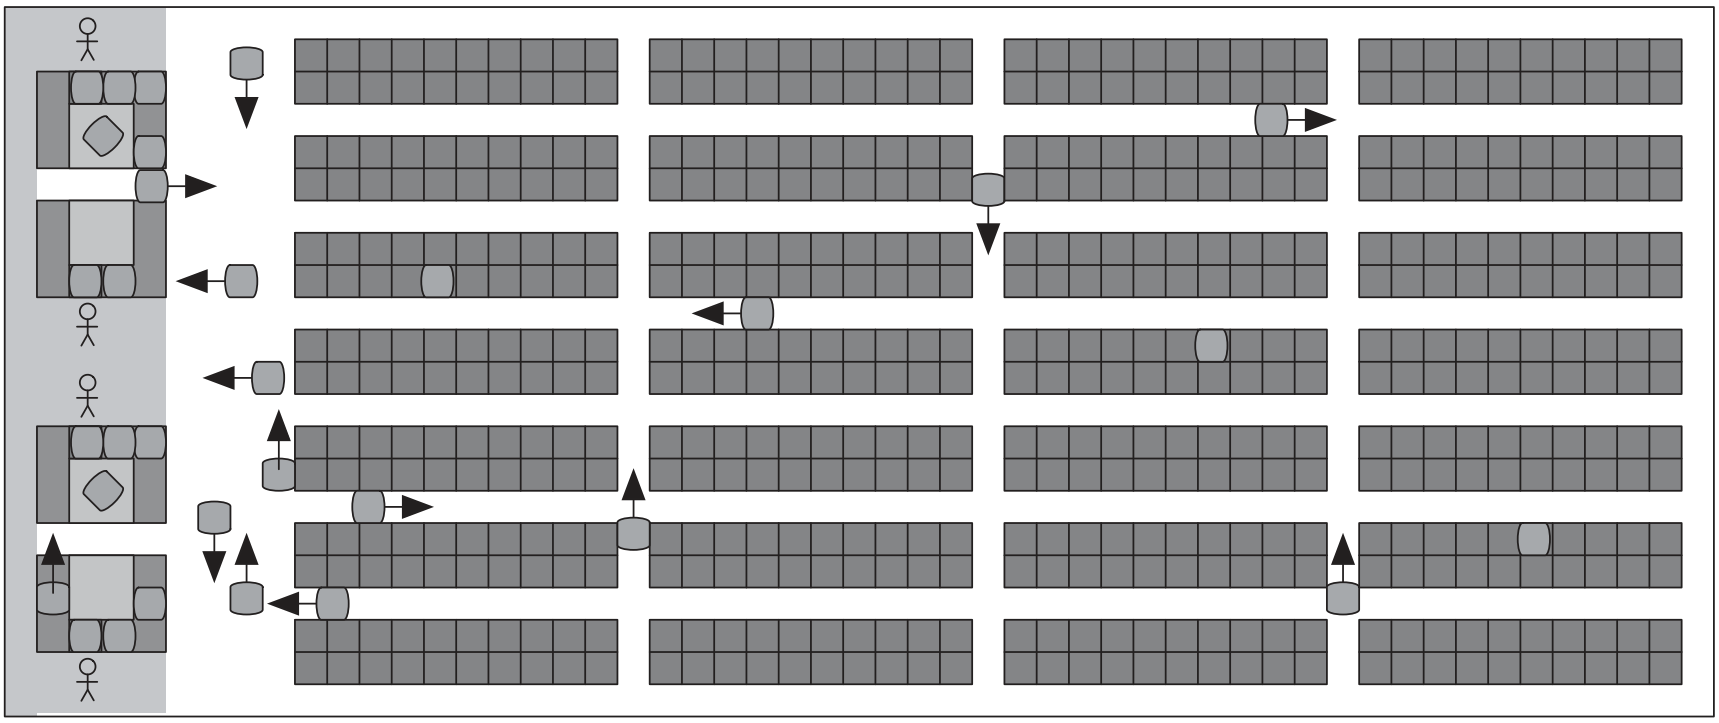
\includegraphics[width=\columnwidth]{Figs/kiva.png}
  \caption{Typical Kiva domain \cite{WDM:AIM:08}.}
  \label{kiva_fig}
\end{figure}

%%%%%%%%%%%%%%%%%%%%%%%%%%%%%%%%%%%%%%%%%%%%%%%%%%%%%%%%%%%%%%%%%%%%%%%%%%%%%%%%%%%%%%%%%%%%%%%%%%%%%%%%%%%%%%%%%%%%%%%%%%%
\section{Definitions}
%%%%%%%%%%%%%%%%%%%%%%%%%%%%%%%%%%%%%%%%%%%%%%%%%%%%%%%%%%%%%%%%%%%%%%%%%%%%%%%%%%%%%%%%%%%%%%%%%%%%%%%%%%%%%%%%%%%%%%%%%%%

We define the MAPF problem formally as follows: We are given a graph $G =
(V,E)$ and a set of $K$ agents $1, \ldots, K$. Each agent $j$ has a unique
start vertex $s^j \in V$ and a unique goal vertex $g^j \in V$. At each time
step, each agent can either move to an adjacent vertex or wait at its current
vertex, both with cost one. A \emph{solution} to a MAPF instance is a set of
\emph{feasible paths}, one path $\{ s^j_0, \ldots, s^j_{T_j}, s^j_{T_j +1},
\ldots \}$ for each agent $j \in \{1,\ldots,K\}$, such that no two paths are
in \emph{collision}. A path for agent $j$ is \emph{feasible} if and only if 1)
it starts at agent $j$'s start vertex, that is, $s^j_0=s^j$; 2) it ends at
agent $j$'s goal vertex and remains there, that is, there exists a lowest
$T_j$ such that $s^j_{T_j}=g^j$ and, for each $t > T_j$, $s^j_t = g^j$; and 3)
every action is a legal move or wait action, that is, for all $t \in \{0,1,
\ldots, T_j-1\} \ , \ (s^j_t,s^j_{t+1}) \in E$ or $s^j_t = s^j_{t+1}$. A
\emph{collision} between the paths of agents $j$ and $k$ is either a
\emph{vertex collision} $(j,k,s,t)$, that is, $s = s^j_t = s^k_t$, or an
\emph{edge collision} $(j,k,s_1,s_2,t)$, that is, $s_1 = s^j_t = s^k_{t+1}$
and $s_2 = s^j_{t+1} = s^k_t$. A constraint is either a vertex constraint or
an edge constraint. A \emph{vertex constraint} $(j,s,t)$ prohibits agent $j$
from occupying $s$ at time step $t$. An \emph{edge constraint} $(j,s_1,s_2,t)$
prohibits agent $j$ from moving from $s_1$ to $s_2$ at time step $t$. The cost
of agent $j$'s path is the number of time steps $T_j$ until it reaches its
goal vertex. Our objective is to minimize the sum $\sum_{j=1}^K T_j$ of the
path costs of all agents, which is a common objective in the literature
\cite{YL:AAAI:13,SSFS:AIJ:15}.

%%%%%%%%%%%%%%%%%%%%%%%%%%%%%%%%%%%%%%%%%%%%%%%%%%%%%%%%%%%%%%%%%%%%%%%%%%%%%%%%%%%%%%%%%%%%%%%%%%%%%%%%%%%%%%%%%%%%%%%%%%%
\section{CBS}
%%%%%%%%%%%%%%%%%%%%%%%%%%%%%%%%%%%%%%%%%%%%%%%%%%%%%%%%%%%%%%%%%%%%%%%%%%%%%%%%%%%%%%%%%%%%%%%%%%%%%%%%%%%%%%%%%%%%%%%%%%%

CBS \cite{SSFS:AIJ:15} is an optimal MAPF algorithm. It performs high-level
and low-level searches. Each node in the high-level search tree (high-level
node) contains a set of constraints and a set of feasible paths (one for each
agent) that respect the set of constraints. The high-level root node has no
constraints. The high-level search of CBS is a best-first search that uses the
costs of the high-level nodes as f-values. The cost of a high-level node is
the sum of the path costs of its paths. When CBS expands a high-level node
$N$, it checks whether the node is a goal node. A high-level node is a
goal node if and only if none of its paths are in collision. If $N$ is a goal
node, then CBS terminates successfully and outputs the paths of the goal node
as solution. Otherwise, at least two paths are in collision, and CBS generates
two high-level children of $N$, called $N_1$ and $N_2$. Both $N_1$ and $N_2$
inherit the constraints of $N$. If the collision is a vertex collision
$(j,k,s,t)$, then CBS adds the constraint $(j,s,t)$ to $N_1$ and the
constraint $(k,s,t)$ to $N_2$. If the collision is an edge collision
$(j,k,s_1,s_2,t)$, then CBS adds the constraint $(j,s_1,s_2,t)$ to $N_1$ and
the constraint $(k,s_2,s_1,t)$ to $N_2$. When CBS generates a high-level node
$N$, it performs a low-level search for each agent independently. The
low-level search for agent $j$ is a (best-first) A* search that ignores all
other agents and finds a minimum-cost path from agent $j$'s start vertex to
its goal vertex that is both feasible and respects the constraints of $N$ that
involve agent $j$.

We use the following notation for all CBS variants: \opt is the cost of an
optimal solution of the MAPF instance. \optna N j is the cost of an optimal
path for agent $j$ that respects the constraints of high-level node $N$.
$\costna N j$ is the cost of the path found by the low-level search.  Let
$\optn N = \sum_{j=1}^K \optna N j$ and $\costn N = \sum_{j=1}^K \costna N j$.
$\lbna N j$ is the minimum $f$-value in the \open list of the low-level search
for agent $j$ after it terminates when high-level node $N$ is generated. Let
$\lbn N = \sum_{j = 1}^K \lbna N j$ and $\lb = \min_{N \in \tiny \open} \lbn
N$ for the \open list of the high-level search.

%%%%%%%%%%%%%%%%%%%%%%%%%%%%%%%%%%%%%%%%%%%%%%%%%%%%%%%%%%%%%%%%%%%%%%%%%%%%%%%%%%%%%%%%%%%%%%%%%%%%%%%%%%%%%%%%%%%%%%%%%%%
\section{ECBS}
%%%%%%%%%%%%%%%%%%%%%%%%%%%%%%%%%%%%%%%%%%%%%%%%%%%%%%%%%%%%%%%%%%%%%%%%%%%%%%%%%%%%%%%%%%%%%%%%%%%%%%%%%%%%%%%%%%%%%%%%%%%

ECBS($w$) \cite{BSSF:SOCS:14} is a bounded-suboptimal MAPF algorithm based on
CBS that is faster than all other bounded-suboptimal MAPF algorithms compared
in \cite{BSSF:SOCS:14}. The high-level and low-level searches of ECBS($w$) are
focal searches \cite{PJ:IEEE:82} instead of best-first searches. A best-first
search maintains an \open list. A focal search also maintains a \focal list,
that contains a subset of the \open list. A best-first search expands the node
with the lowest f-value in the \open list. A focal search, on the other hand,
expands a node in the \focal list that is determined by a user-provided
tie-breaking criterion. The low-level searches of ECBS($w$) for agent $j$ are
focal searches with a \focal list that contains all low-level nodes $n \in
\open$ in the \open list of the low-level search such that $f(n) \leq w
f_{min}$, where $w > 1$ is a user-provided parameter and $f_{min}$ is the
lowest f-value of any node in the \open list. We refer to a focal search with
such a \focal list as \emph{regular focal search}. The high-level search of
ECBS($w$) is a focal search with a \focal list that contains all high-level
nodes $N \in \open$ in the \open list of the high-level search such that
$\costn N \leq w \lb$. The low-level searches and the high-level search use
their flexibility in deciding which nodes to expand to reduce the number of
collisions by using appropriate tie-breaking criteria. ECBS($w$) is
$w$-suboptimal if its low-level searches are allowed to re-expand nodes to
lower the f-values of the nodes.

%%%%%%%%%%%%%%%%%8%%%%%%%%%%%%%%%%%%%%%%%%%%%%%%%%%%%%%%%%%%%%%%%%%%%%%%%%%%%%%%%%%%%%%%%%%%%%%%%%%%%%%%%%%%%%%%%%%%%%%%%%%%
\section{Incorporating Highways}
%%%%%%%%%%%%%%%%%%%%%%%%%%%%%%%%%%%%%%%%%%%%%%%%%%%%%%%%%%%%%%%%%%%%%%%%%%%%%%%%%%%%%%%%%%%%%%%%%%%%%%%%%%%%%%%%%%%%%%%%%%%

\begin{figure*}[t]
%\centerfloat
  \begin{subfigure}[b]{0.12\textwidth}
    \centering
	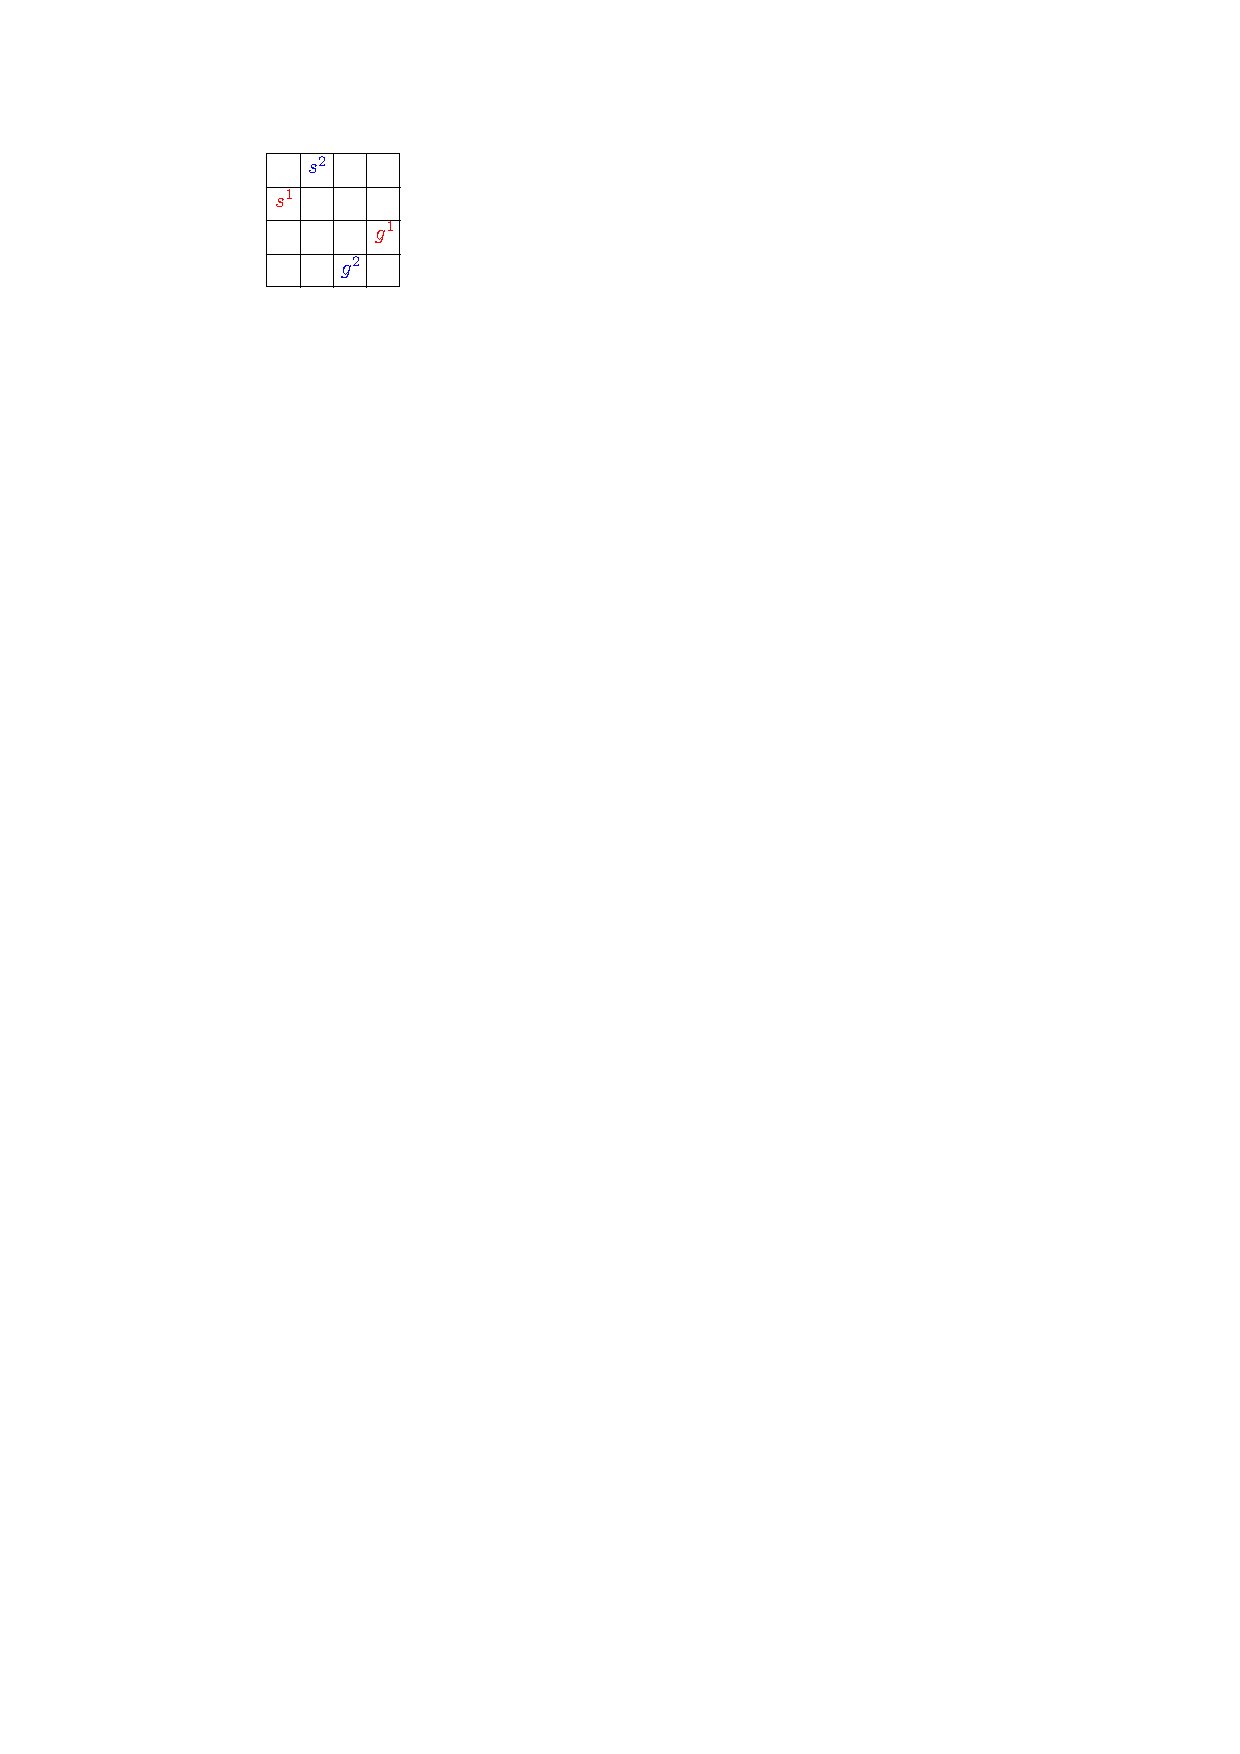
\includegraphics[width=0.95\textwidth]{Figs/example1_map.pdf}
    \caption{}
  \end{subfigure}
  \begin{subfigure}[b]{0.12\textwidth}
	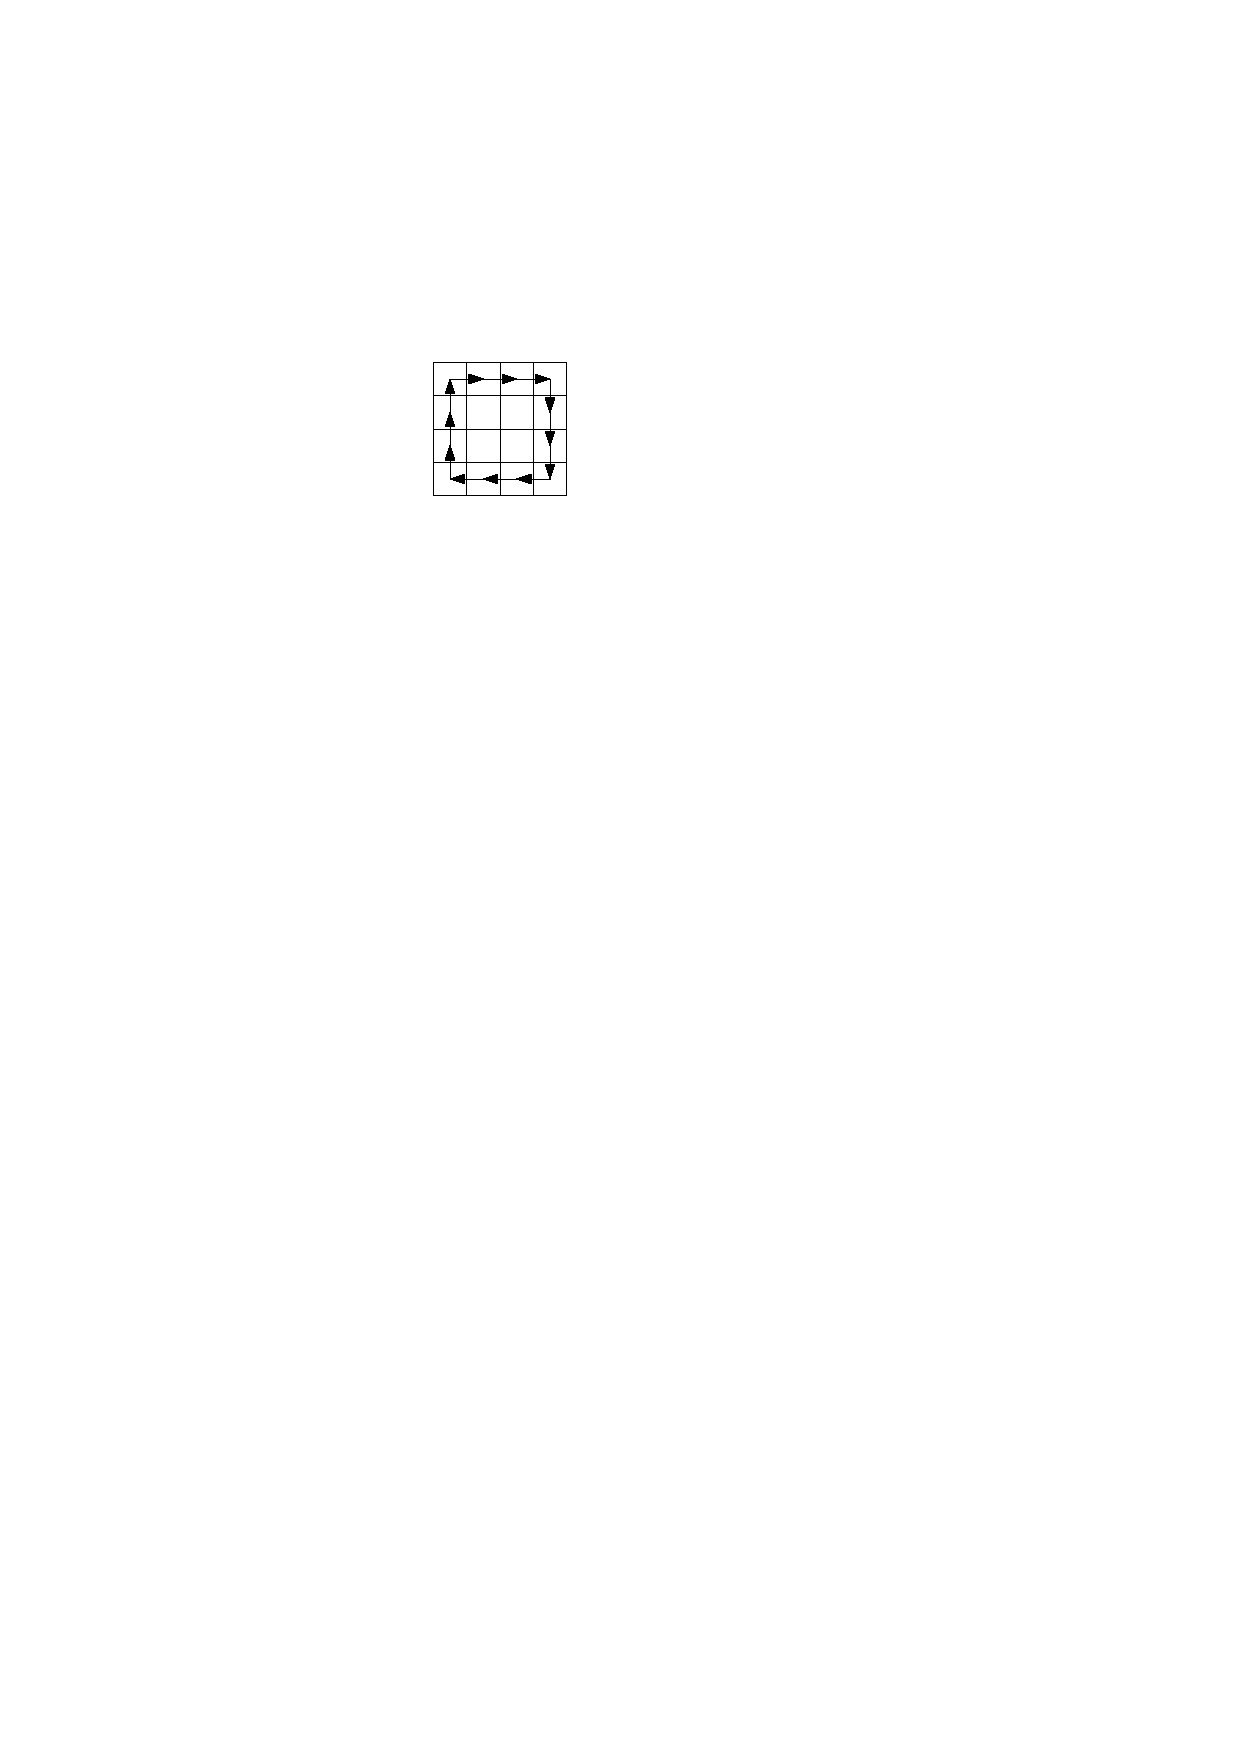
\includegraphics[width=0.95\textwidth]{Figs/example1_EG.pdf}
    \caption{}
  \end{subfigure}
  \begin{subfigure}[b]{0.12\textwidth}
    \centering
	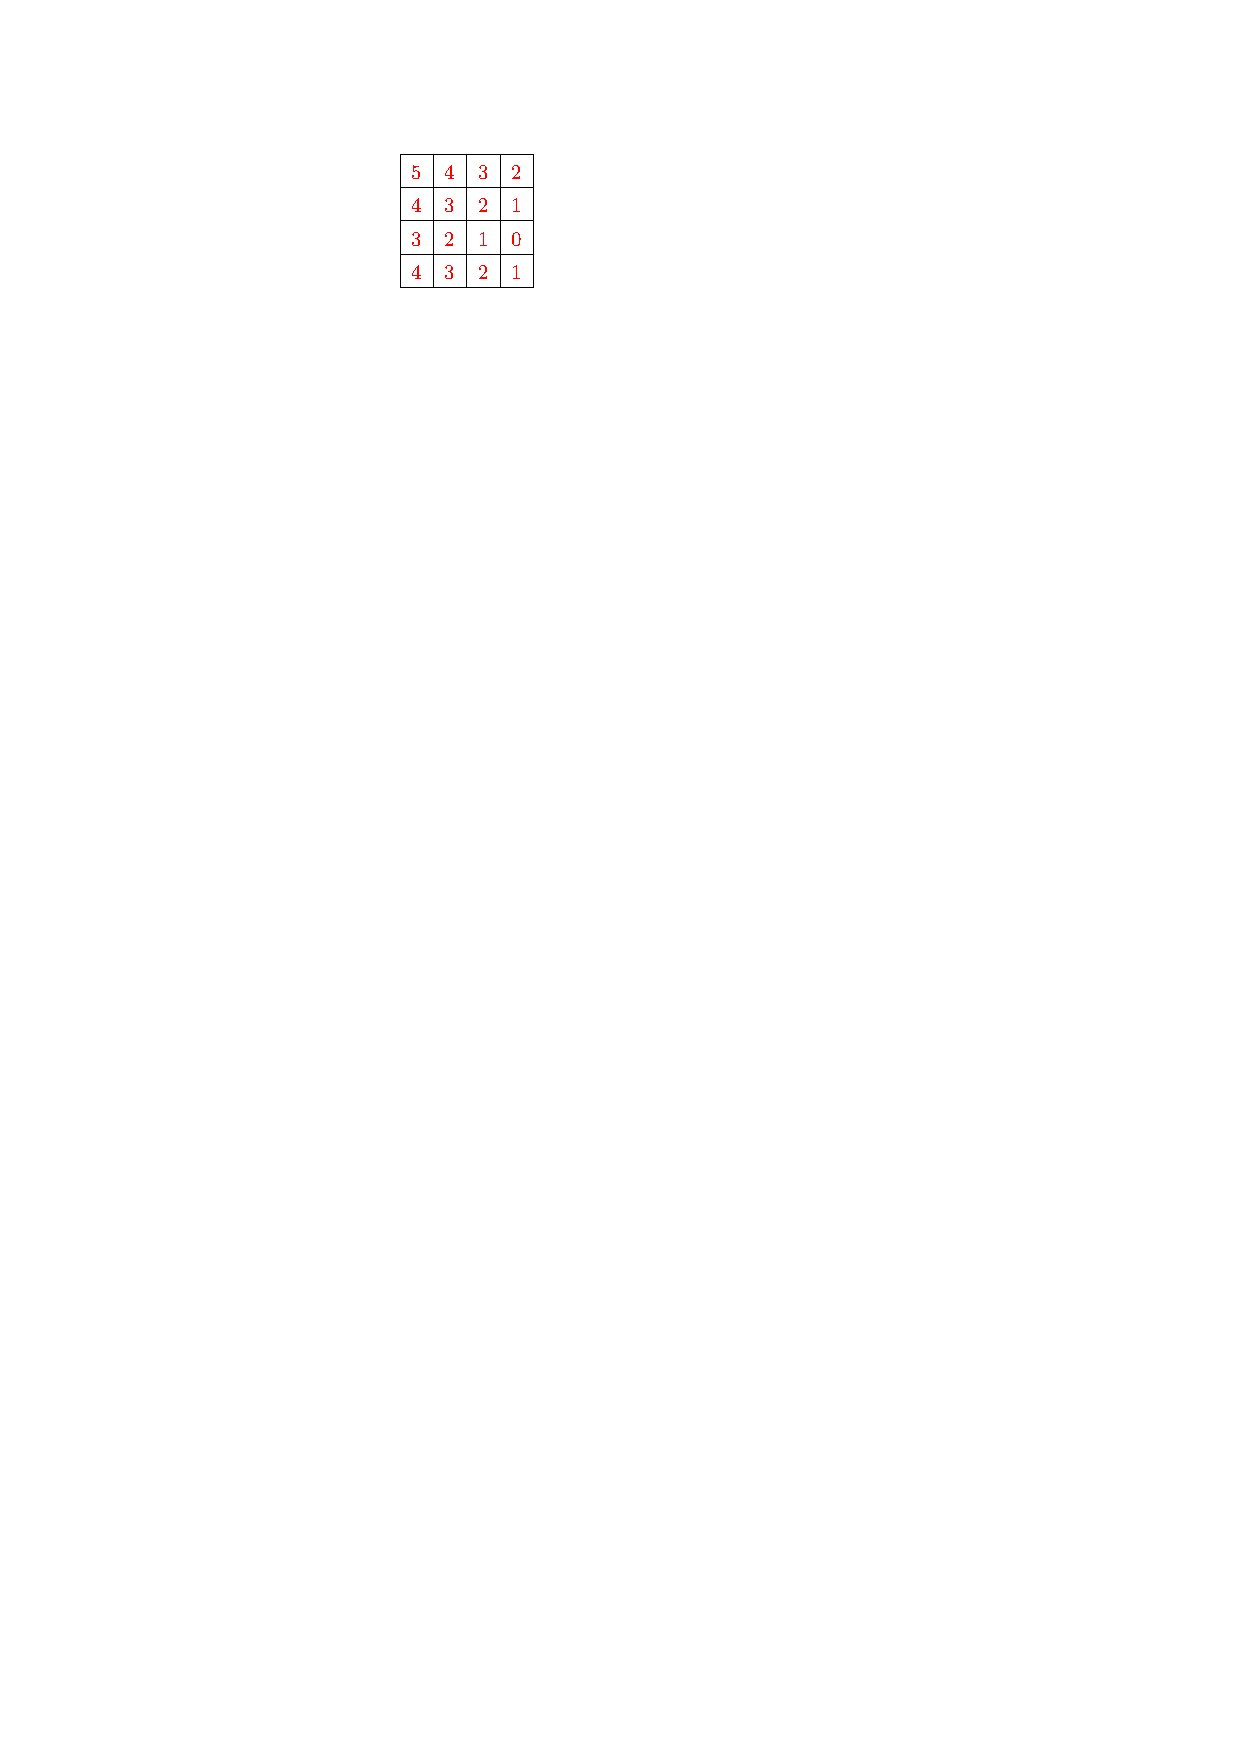
\includegraphics[width=0.95\textwidth]{Figs/example1_a1_h.pdf}
    \caption{}
  \end{subfigure}
  \begin{subfigure}[b]{0.12\textwidth}
	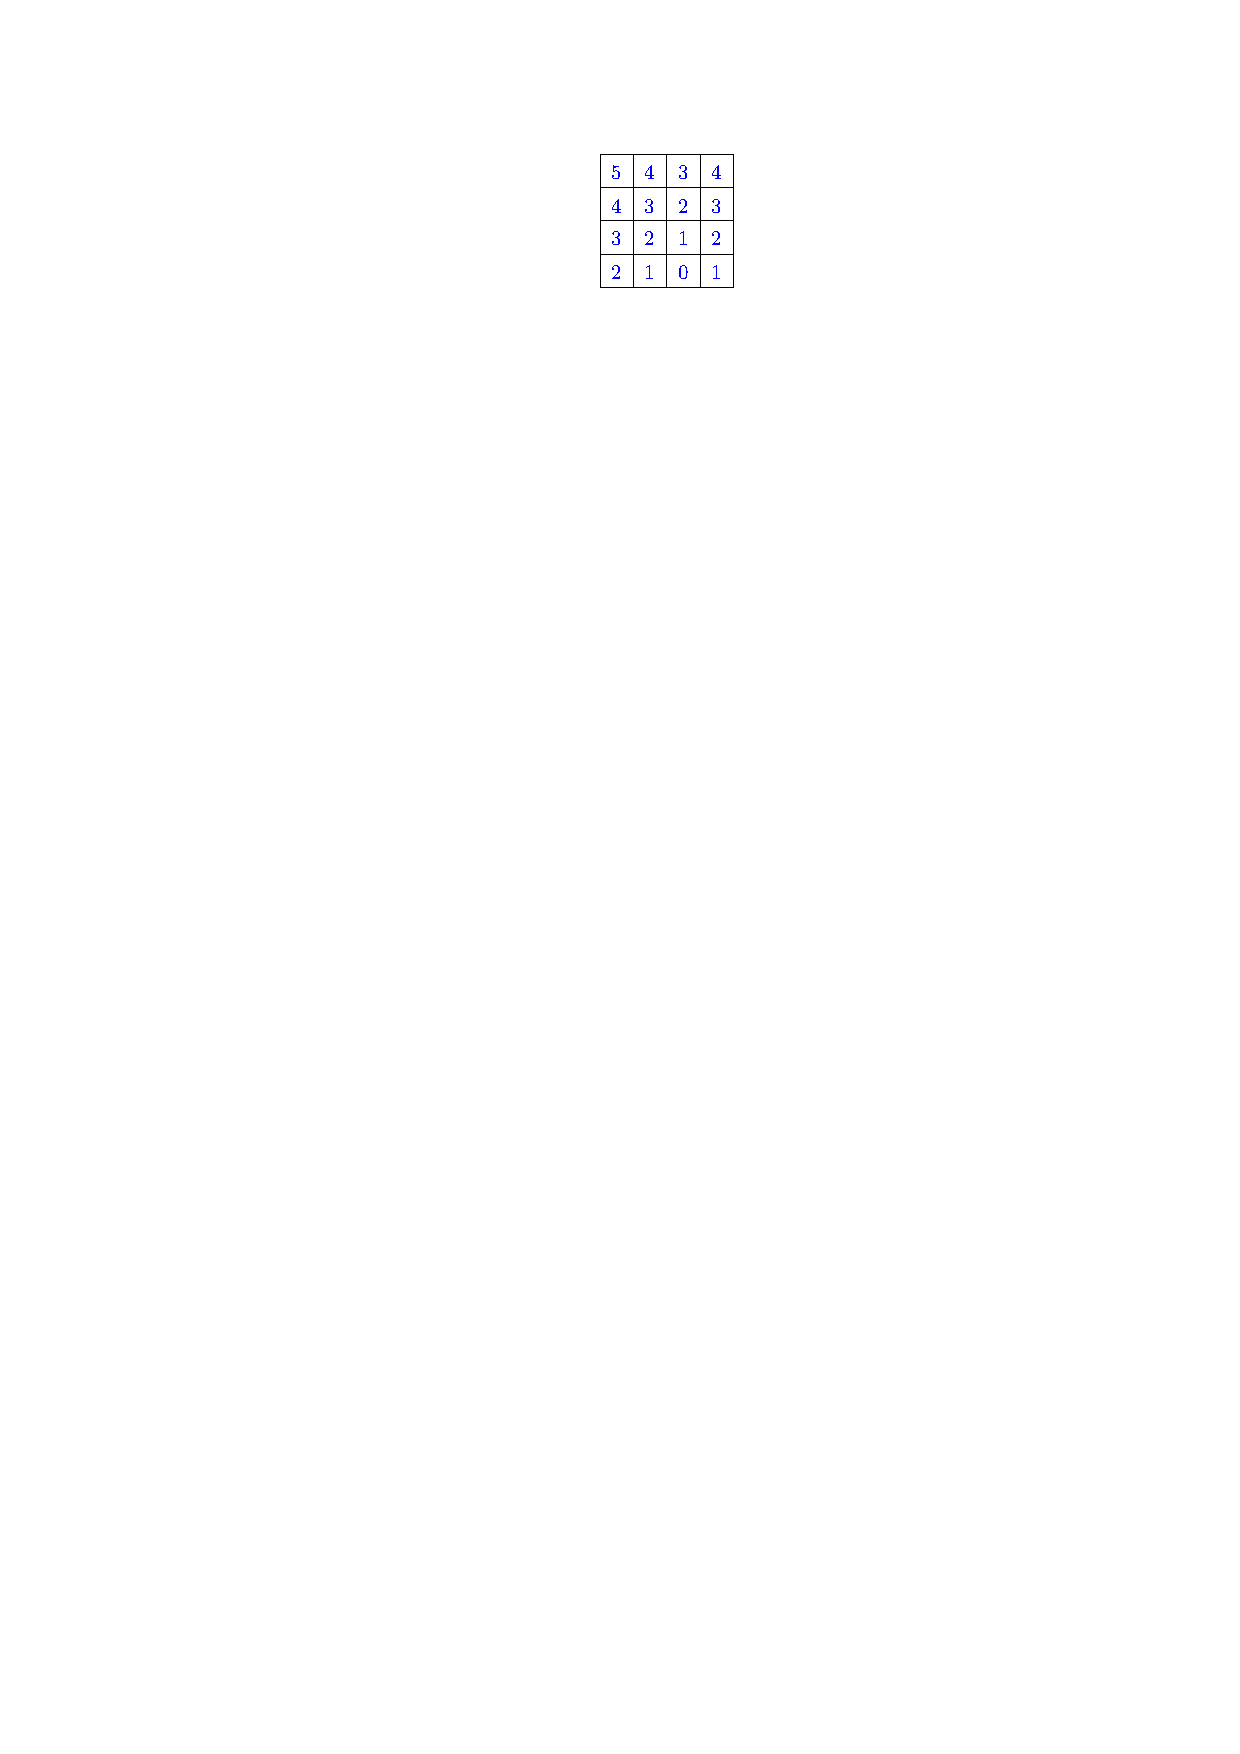
\includegraphics[width=0.95\textwidth]{Figs/example1_a2_h.pdf}
    \caption{}
  \end{subfigure}
  \begin{subfigure}[b]{0.12\textwidth}
    \centering
	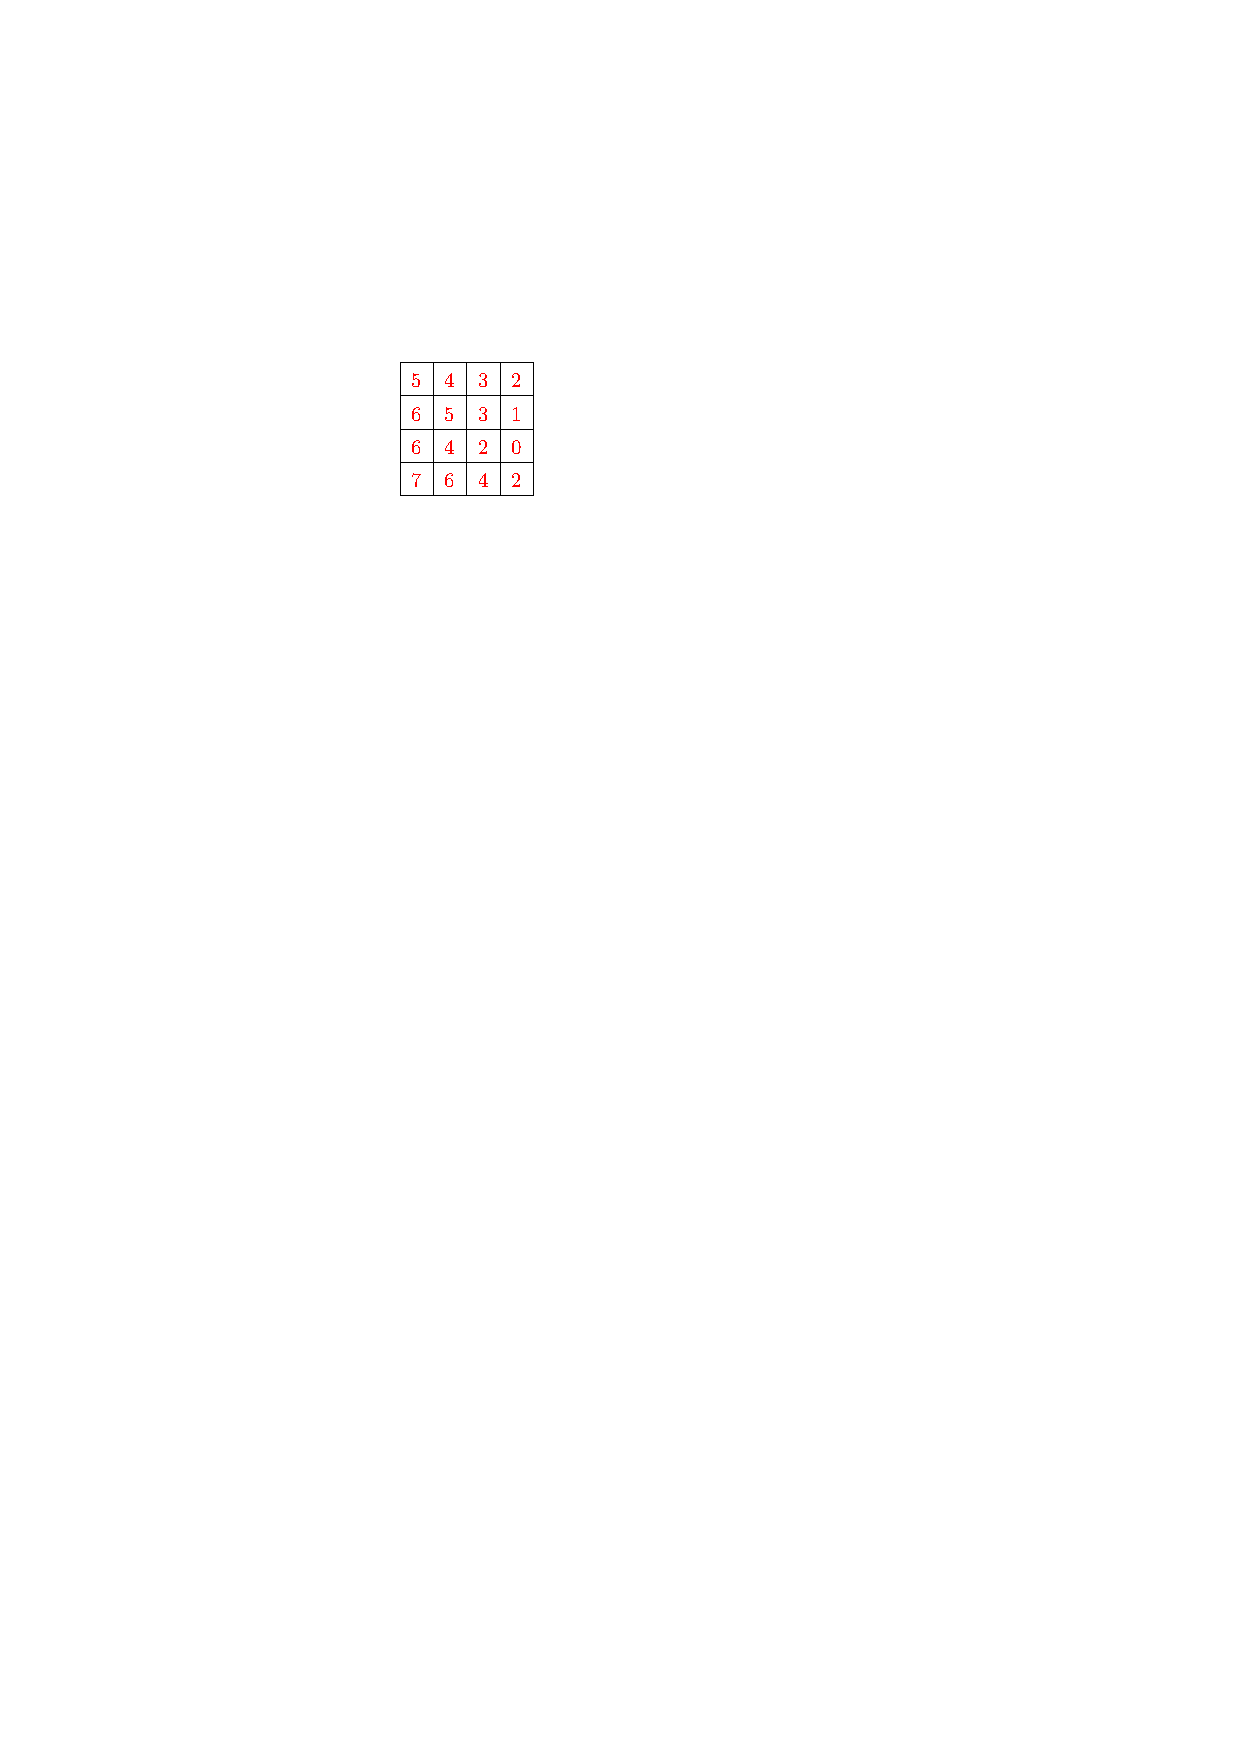
\includegraphics[width=0.95\textwidth]{Figs/example1_a1_h_EG.pdf}
    \caption{}
  \end{subfigure}
  \begin{subfigure}[b]{0.12\textwidth}
	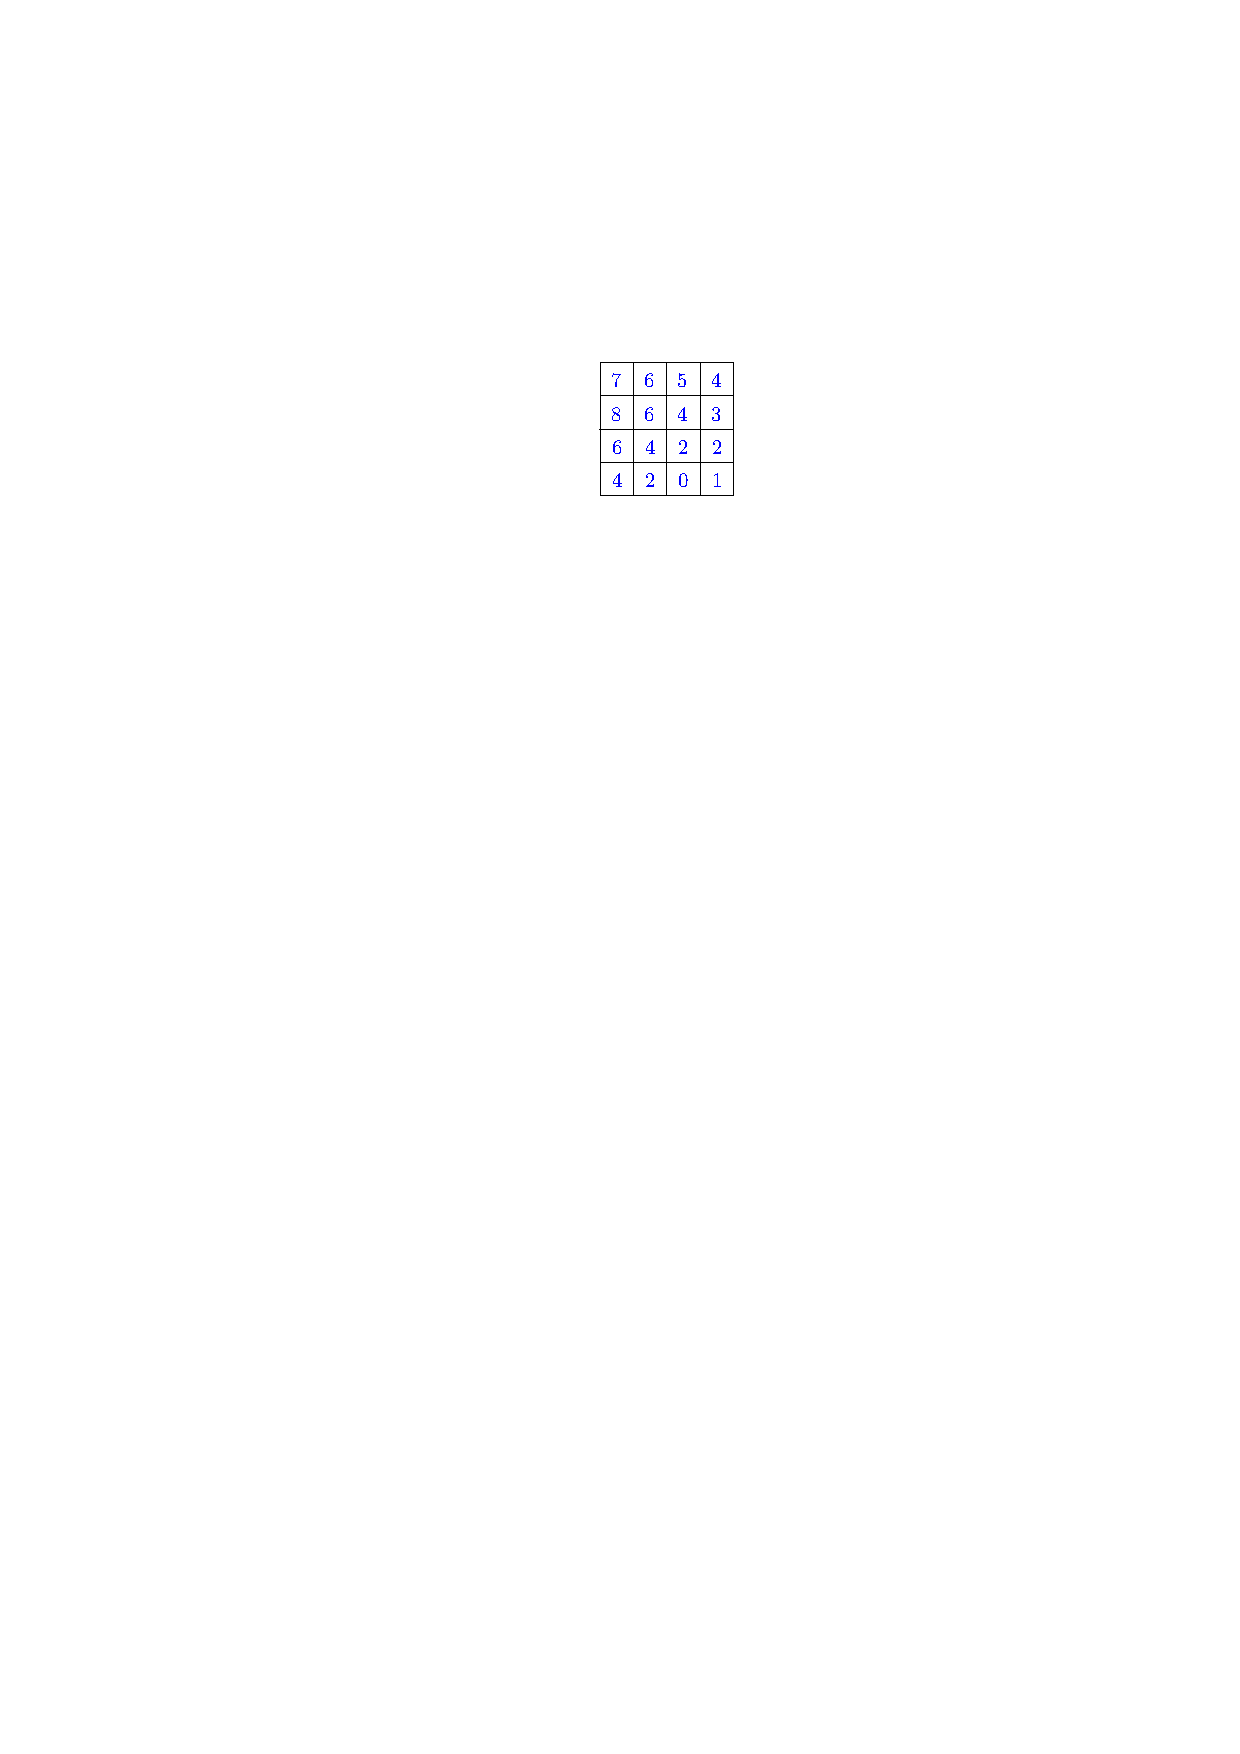
\includegraphics[width=0.95\textwidth]{Figs/example1_a2_h_EG.pdf}
    \caption{}
  \end{subfigure}
  \begin{subfigure}[b]{0.12\textwidth}
    \centering
	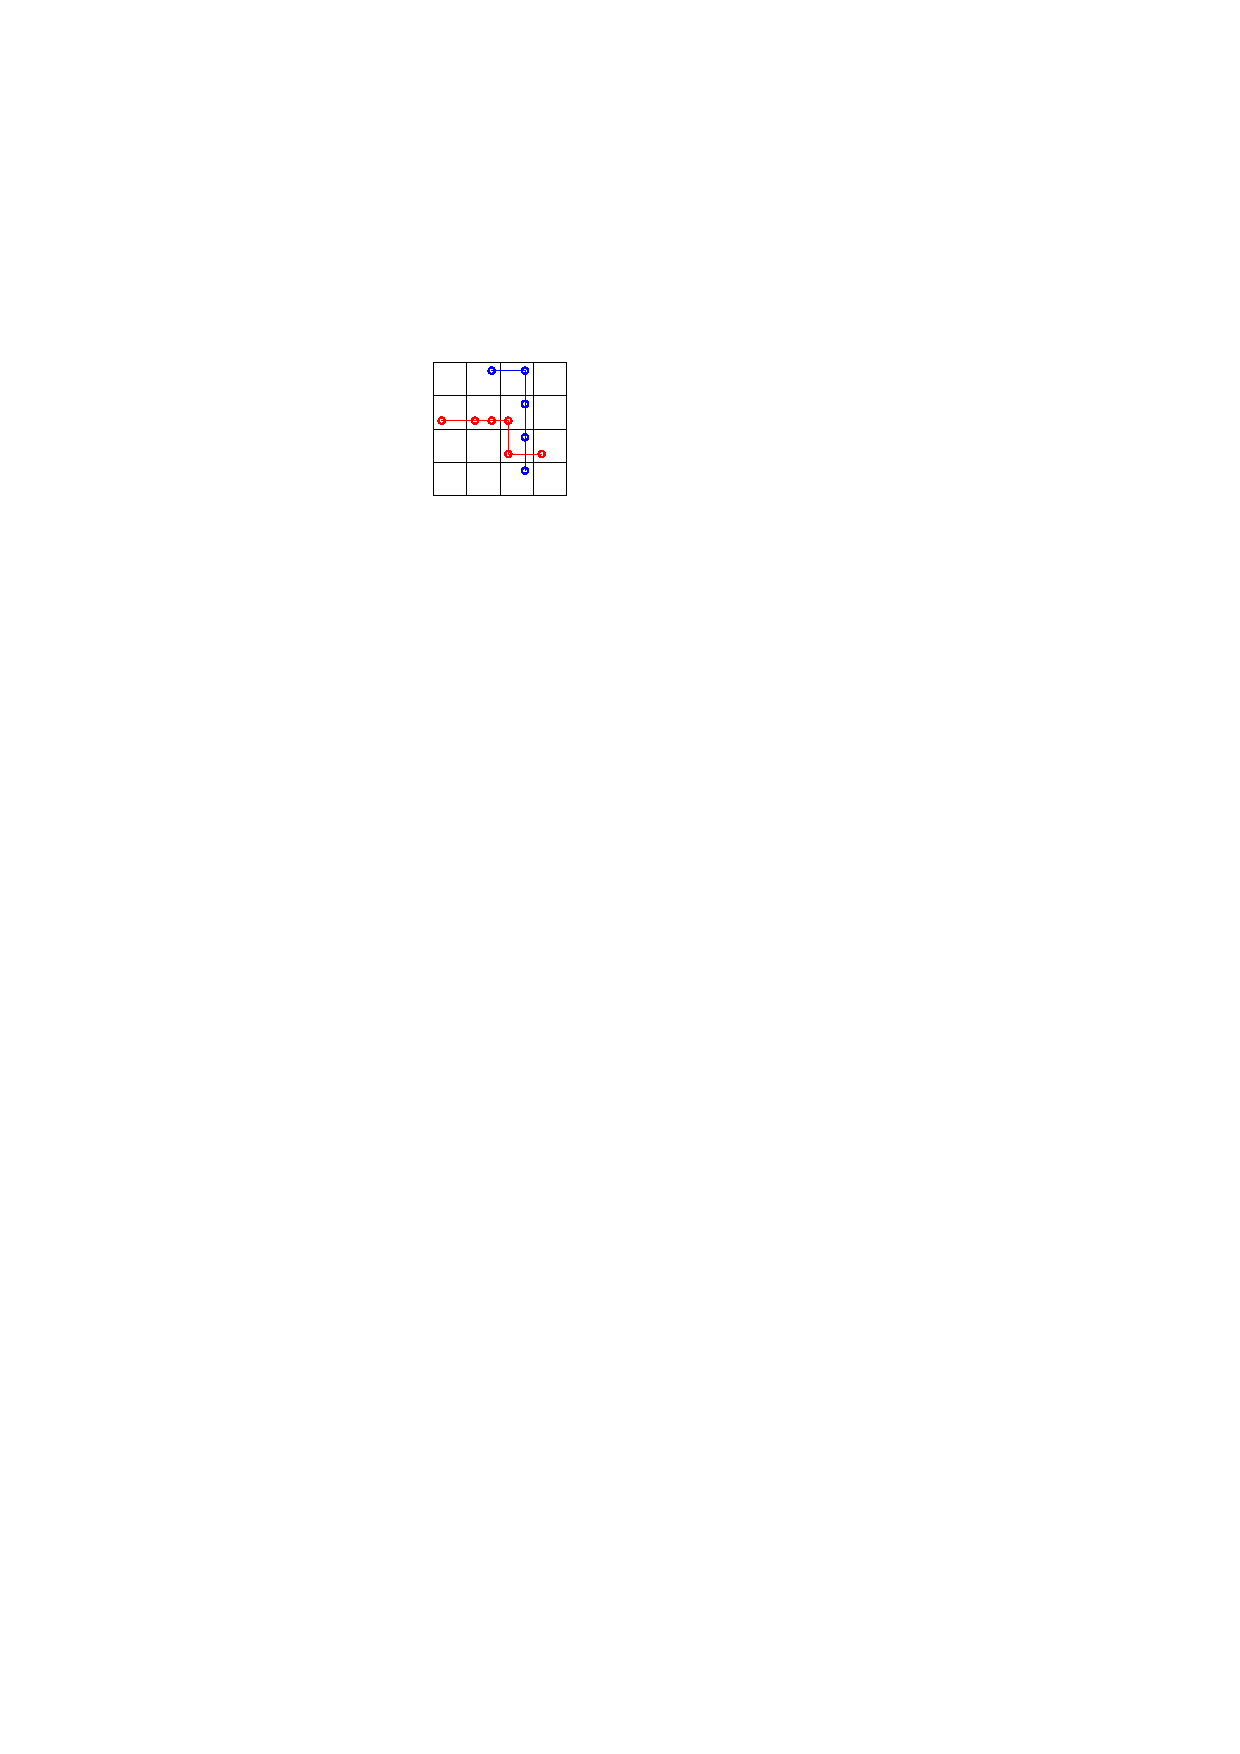
\includegraphics[width=0.95\textwidth]{Figs/example1_paths.pdf}
    \caption{}
  \end{subfigure}
  \begin{subfigure}[b]{0.12\textwidth}
	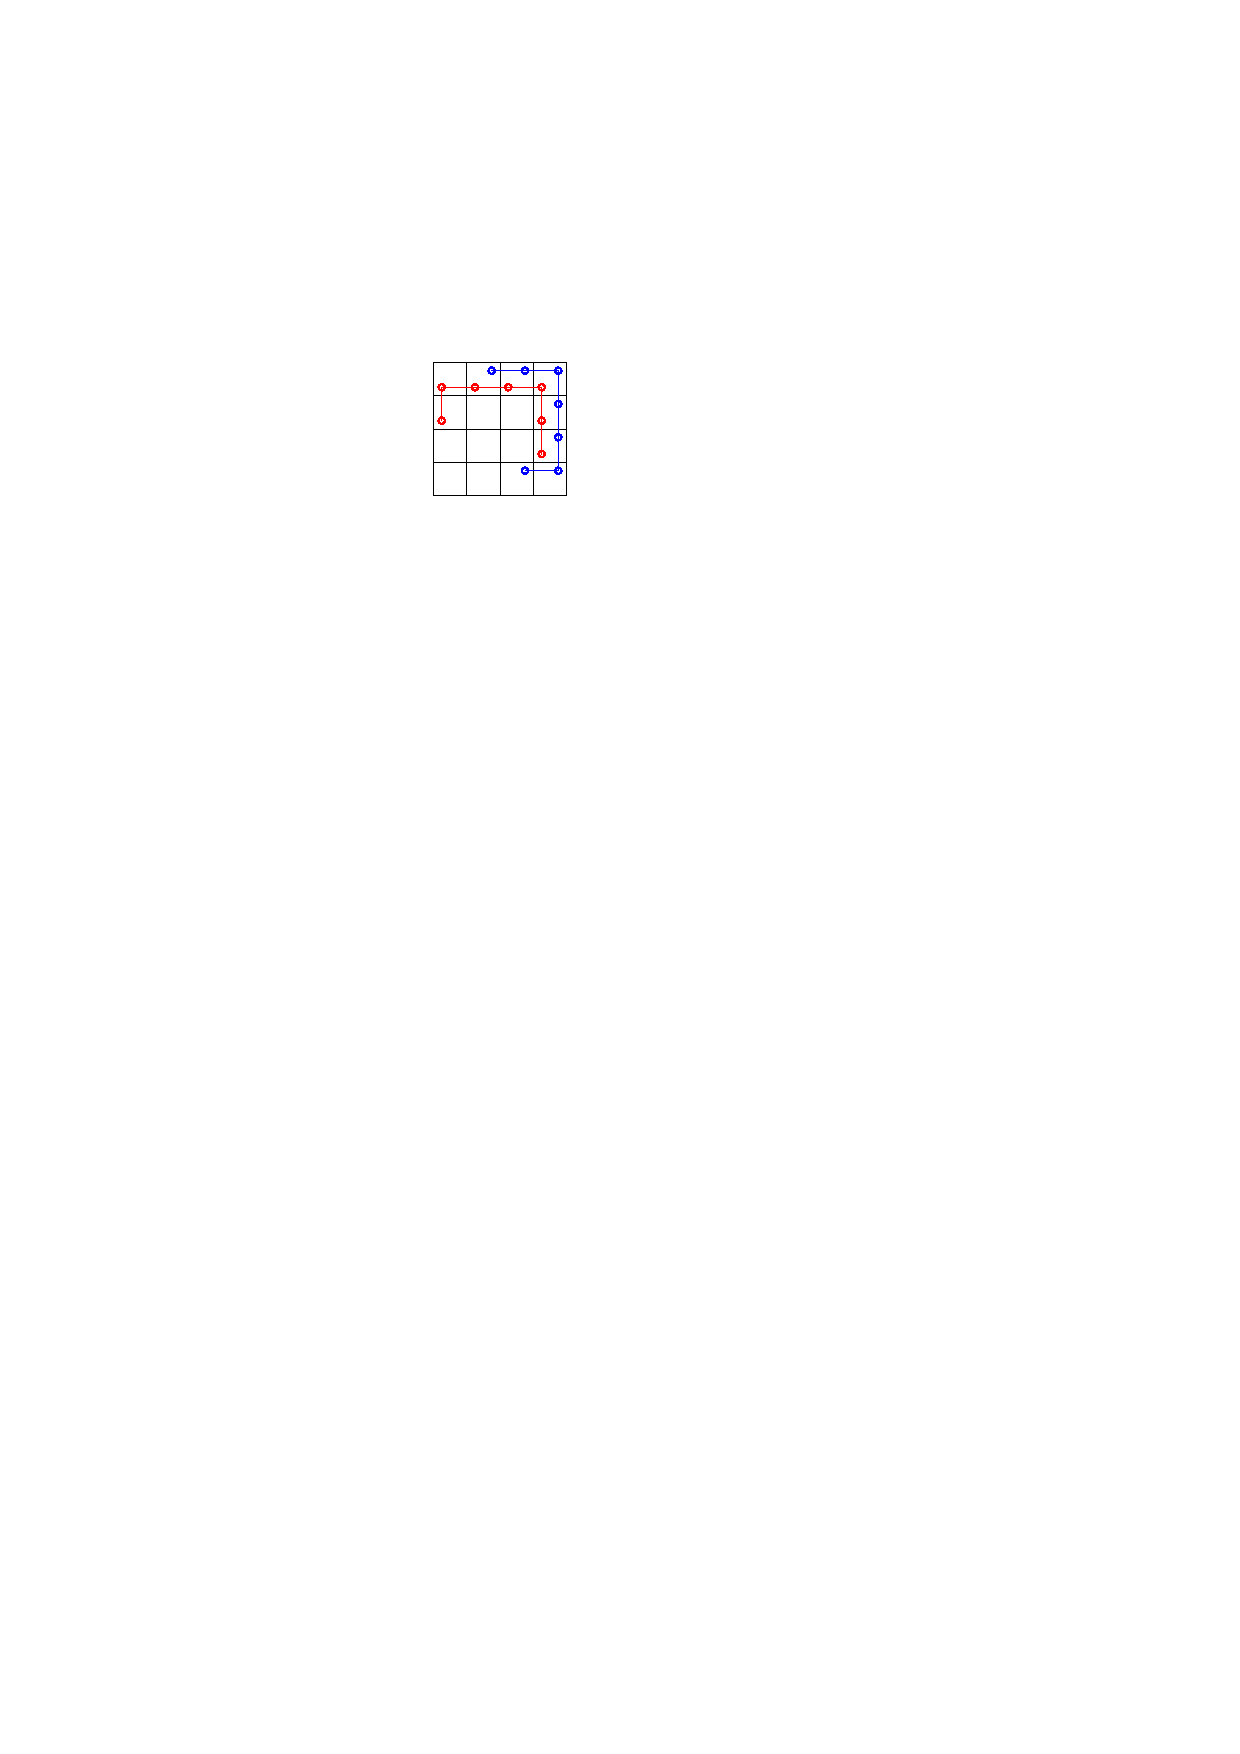
\includegraphics[width=0.95\textwidth]{Figs/example1_EG_paths.pdf}
    \caption{}
  \end{subfigure}
  \caption{Differences between CBS and CBS+HWY($2.0$) in a pathological domain
    where CBS is extremely inefficient. (a) shows the start and goal vertices
    for the two agents. (b) shows the highway. (c) and (d) show the
    shortest-path heuristic values for agents $1$ and $2$, respectively. (e)
    and (f) show the highway heuristic values for agents $1$ and $2$,
    respectively. (g) shows the paths found by CBS. (h) shows the paths found
    by CBS+HWY($2.0$). Each dot represent a time step. Two dots in the same
    cell thus represent a wait action.}
    \label{example1_fig}
\end{figure*}

The low-level searches of all CBS variants when high-level node $N$ is
generated typically use the \emph{shortest-path heuristic values} $h^j(s)$,
that is, the perfect heuristic values for agent $j$ when all constraints of
$N$ are ignored, defined formally as { \small
\begin{align*}
\label{eq:h_def}
h^j(s) = \min_{\pi} \sum_{(s_i,s_{i+1}) \in \pi} 1,
\end{align*}
} where $\pi = \{ s, \ldots, g^j \}$ is a feasible path that takes agent $j$
from $s$ to its goal vertex. The shortest-path heuristic values can be
computed quickly and are more informed than the Manhattan distance heuristic
values, which is why CBS variants use them to guide their low-level
searches. The low-level searches of Weighted-CBS and M* for agent $j$ are
weighted A* searches with $w h^j(s)$ as heuristic values, that is, the
heuristic values $h^j(s)$ are inflated uniformly by $w$. The low-level
searches of ECBS($w$) for agent $j$ are regular focal searches with a \focal
list that contains all nodes $n \in \open$ in the \open list of the low-level
search such that $f(n) = g(n) + h^j(n) \leq w f_{min}$, where $f_{min}$ is the
lowest f-value of any node in the \open list.

Increasing $w$ allows for longer paths, which provides agents with the
flexibility to avoid collisions by moving around other agents in domains with
few agents. The high-level searches of CBS variants then have to resolve fewer
collisions and can terminate earlier, potentially reducing the runtimes of the
CBS variants. However, this also makes the agents spread out more, which can
in turn result in a higher number of additional collisions in domains with
many agents and increase the runtimes of the CBS variants. Thus, larger values
of $w$ are not necessarily beneficial.

We therefore develop bounded-suboptimal MAPF algorithms that exploit the
problem structure of a given MAPF instance by finding paths for the agents
that include edges from user-provided sets of edges (called highways).
Highways are used in the context of transportation as a means to provide
guidance for vehicles to avoid collisions with vehicles that travel in the
opposite direction.  Our algorithms inflate heuristic values non-uniformly in
a way that encourages path finding to return paths that include the edges of
the highways, which encourages a global behavior of the agents that avoids
collisions. Highways are a convenient way for users to influence the heuristic
values and, since the runtimes of CBS variants increase with the number of
collisions, have the potential to speed them up. We use the ideas behind
experience graphs \cite{PCCL:RSS:12}, which were developed to speed up motion
planning, to derive suitable heuristic values.

Formally, a \emph{highway} is a subgraph $G_{hwy}=(V_{hwy},E_{hwy})$ of the
given graph $G=(V,E)$. The low-level searches use the \emph{highway heuristic
  values} $h^j_{hwy}(s)$ for the user-provided parameter $w>1$ (that
determines the level of encouragement for path finding to return paths that
include the edges of the highway), defined formally as
{ \small
\begin{align*}
h^j_{hwy}(s) = \min_{\pi} \sum_{(s_i,s_{i+1}) \in \pi} \left\{
\begin{array}{rl}
 1 & \text{if} \ (s_i,s_{i+1}) \in E_{hwy} \\
 w & \text{otherwise,}
\end{array}
\right.
\end{align*}
}
where $\pi = \{ s, \ldots, g^j \}$ is a feasible path that takes agent $j$
from $s$ to its goal vertex. We can easily adapt the highway heuristic values
to graphs with non-uniform edge costs.

\begin{proposition}
  For all agents $j$ and states $s$, $h^j(s) \leq h^j_{hwy}(s) \leq w h^j(s)$.
\label{lm:h_hwy_subopt}
\end{proposition}

Heuristic values $h(s)$ are \emph{$w$-admissible} if and only if $0 \leq h(s)
\leq w opt(s)$ for each state $s$, where $opt(s)$ is the cost of an optimal
solution for start vertex $s$. Thus, the heuristic values $h^j_{hwy}(s)$ are
$w$-admissible according to Proposition \ref{lm:h_hwy_subopt} since the
shortest-path heuristic values are admissible.

Figure \ref{example1_fig}(a) shows a MAPF instance as an example. The
shortest-path heuristic values for agents 1 and 2 are shown in (c) and (d),
respectively. The highway heuristic values for agents 1 and 2 are shown in (e)
and (f), respectively, for $w=2$ and the highway shown in (b). For instance,
the shortest-path heuristic value for agent $1$ and the cell in row 2 and
column 3 is $2$ (corresponding to moving east and south, each with cost one)
while the highway heuristic value is $3$ (corresponding to moving east with
cost two and then following the highway south with cost one).

\subsection{Collision-Based Search with Highways}

Our first bounded-suboptimal MAPF algorithm, called CBS+HWY($w$), is a version
of CBS whose low-level searches use the highway heuristic values with
parameter $w$ instead of the shortest-path heuristic values.

\begin{theorem}
  CBS+HWY($w$) is $w$-suboptimal.
\end{theorem}

\begin{proof}
  Let $M$ be any high-level node in the \open list of the high-level search of
  CBS+HWY($w$) that contains an optimal solution of the MAPF instance (that
  is, $\optn M = \opt$). Such an $M$ exists according to Lemma 2
  of~\cite{SSFS:AIJ:15}. The low-level searches of CBS+HWY($w$) use
  $w$-admissible heuristic values according to Lemma
  \ref{lm:h_hwy_subopt}. The low-level search for agent $j$ when high-level
  node $M$ is generated thus is guaranteed to find a path with cost at most $w
  \optna M j$, that is, $\costna M j \leq w \optna M j$. The proof is
  identical to the one that proves the suboptimality guarantee of Weighted-A*
  \cite{P:AI:70}. Consequently, $\costn M \leq w \optn M = w \opt$. The
  high-level search of CBS+HWY($w$) is a best-first search and can thus never
  expand a high-level goal node with a cost of more than $w \opt$. Thus,
  CBS+HWY($w$) is $w$-suboptimal.
\end{proof}

\begin{table}[h]
\resizebox{\columnwidth}{!}{
\begin{tabular}{|c|c|cccc|cccc|}
\hline
\textbf{}        & \textbf{CBS} & \multicolumn{4}{c|}{\textbf{CBS+HWY($w$)}}                & \multicolumn{4}{c|}{\textbf{ECBS($w$)}}                   \\
\textbf{$w$}       & \textbf{-}   & \textbf{1.1} & \textbf{1.2} & \textbf{1.5} & \textbf{2.0} & \textbf{1.1} & \textbf{1.2} & \textbf{1.5} & \textbf{2.0} \\ \hline
\textbf{HL-Exp}  & 7            & 7            & 7            & 3            & 1          & 7            & 3            & 1            & 1          \\
\textbf{HL-Gen}  & 13           & 13           & 13           & 5            & 1          & 13           & 5            & 1            & 1          \\
\textbf{LL-Exp}  & 70           & 70           & 70           & 30           & 12         & 70           & 30           & 9            & 9          \\
\textbf{LL-Gen}  & 277          & 277          & 277          & 115          & 31         & 277          & 115          & 33           & 33         \\
\textbf{SolCost} & 9            & 9            & 9            & 9            & 12         & 9            & 9            & 9            & 9          \\ \hline
\end{tabular}
}
\caption{Expanded and generated nodes and solution costs for CBS, CBS+HWY($w$), and
  ECBS($w$) for the example in Figure \ref{example1_fig}.}
\label{tbl:example1}
\end{table}

Figures \ref{example1_fig}(g) and (h) show the paths found by CBS and
CBS+HWY($2.0$), respectively, for the example in Figure \ref{example1_fig}(a).
The value of $w = 2.0$ is high enough to make both agents travel along the
outer ring to their respective goal vertices. We ran CBS and, for each $w \in
\{ 1.1, 1.2, 1.5, 2.0 \}$, CBS+HWY($w$) and ECBS($w$) on the example in Figure
\ref{example1_fig}. We ran all experiments on a computer with a 3.2GHz Intel
Core i7 CPU and 8GBytes of RAM. Table \ref{tbl:example1} shows the number of
expanded and generated nodes by the high-level and low-level searches (HL-Exp,
LL-Exp, HL-Gen, and LL-Gen, respectively) and the solution costs
(SolCost). The paths found by the low-level searches of CBS+HWY($2.0$) avoid
the inevitable collision of the optimal paths of the two agents when there are
no constraints, which explains why CBS+HWY($2.0$) expands fewer nodes than CBS
although it has a higher solution cost. However, comparing a
bounded-suboptimal MAPF algorithm, like CBS+HWY($2.0$), with an optimal one,
like CBS, is like comparing apples and oranges. Comparing two
bounded-suboptimal MAPF algorithms with the same suboptimality bound, like
CBS+HWY($2.0$) and ECBS($2.0$), is fairer.  Unfortunately, ECBS($2.0$) expands
fewer nodes than CBS+HWY($2.0$) and finds a solution of lower cost. However,
the example is too simple. The number of agents is low, and a single wait
action by one of the two agents prevents the collision of their paths.

\begin{figure*}[t]
%\centerfloat
  \centering
	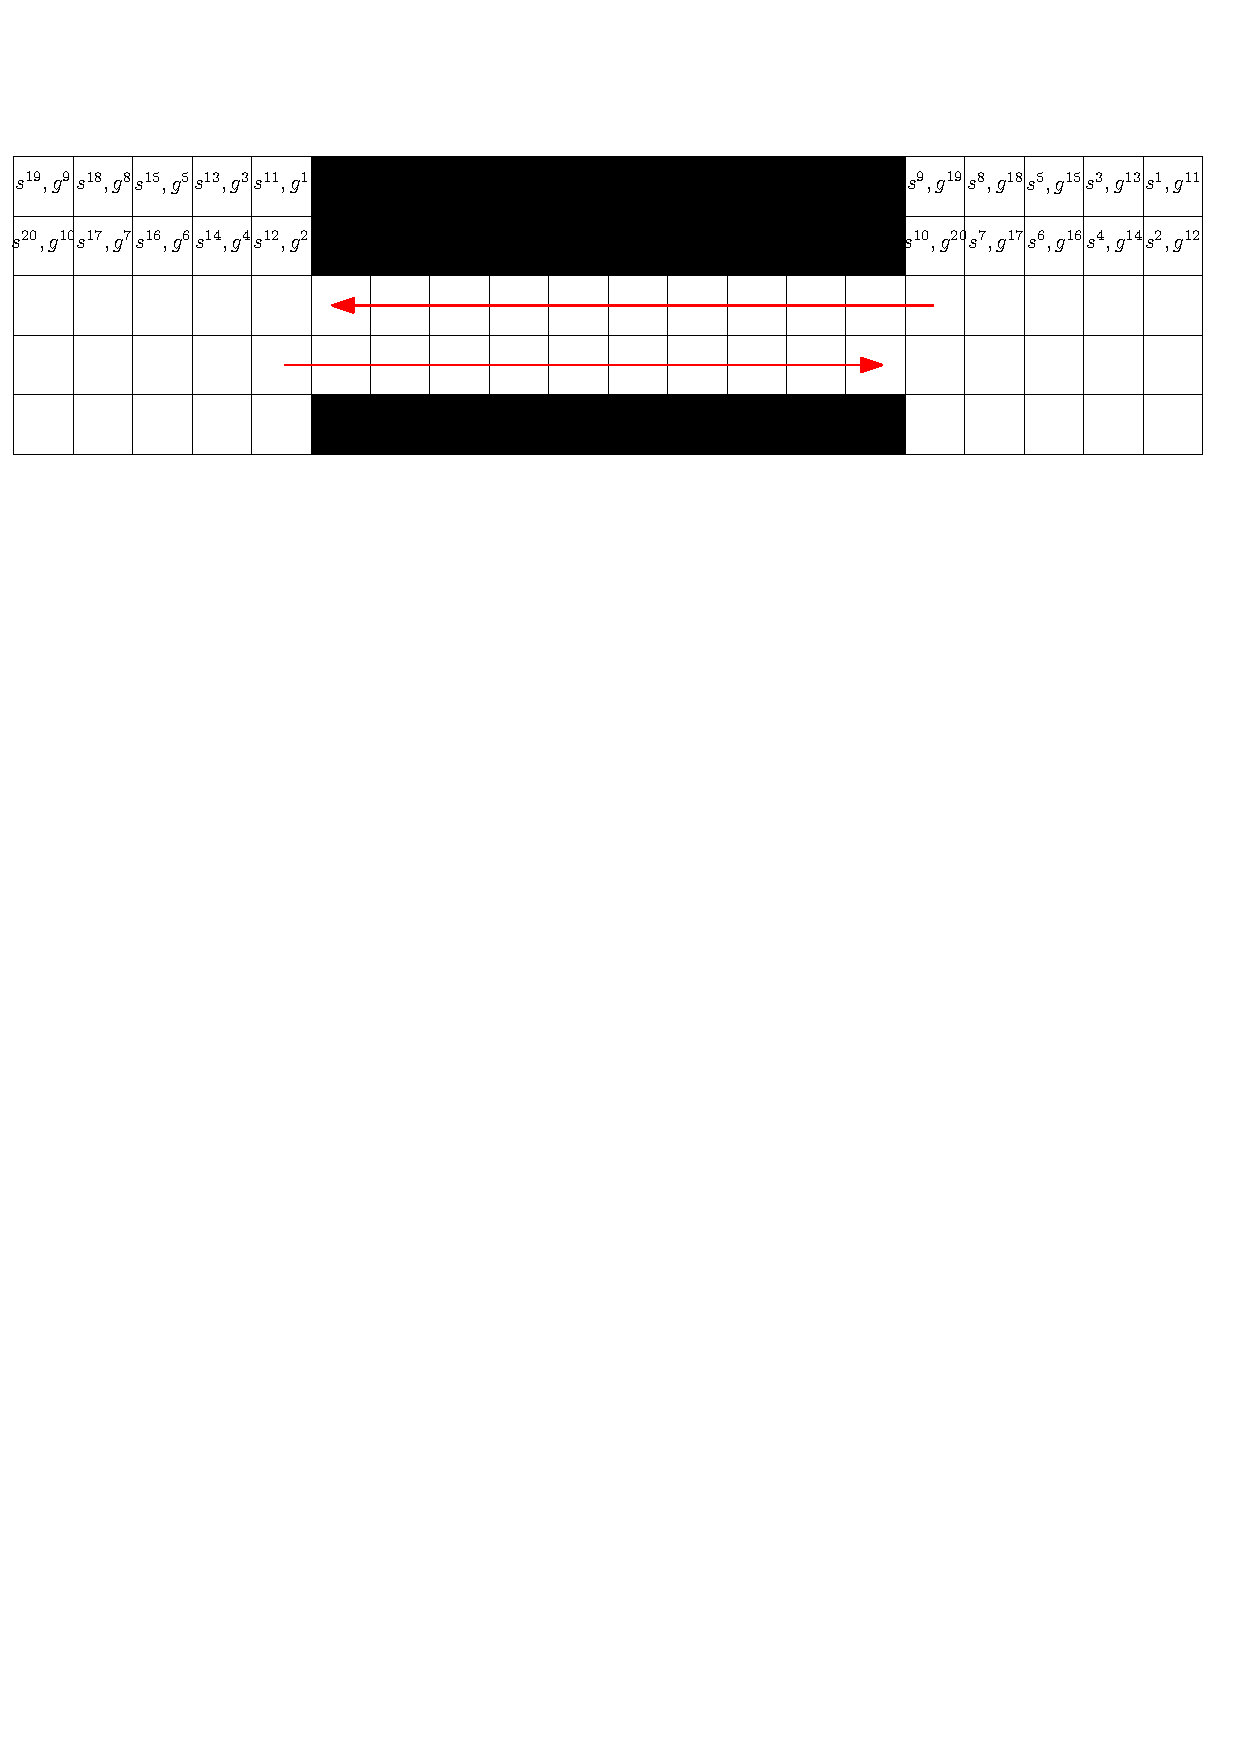
\includegraphics[width=0.75\textwidth]{Figs/example2.pdf}
  \caption{Corridor example on which we compare CBS+HWY($w$) and ECBS($w$).}
  \label{example2_fig}
\end{figure*}

\begin{table}[h]
  \centering
\resizebox{0.37\textwidth}{!}{
\begin{tabular}{|c|cc|cc|}
\hline
\multicolumn{1}{|c|}{\textbf{}}  & \multicolumn{2}{c|}{\textbf{CBS+HWY($w$)}}       & \multicolumn{2}{c|}{\textbf{ECBS($w$)}} \\
\multicolumn{1}{|c|}{\textbf{$w$}} & \textbf{1.5} & \multicolumn{1}{c|}{\textbf{2.0}} & \textbf{1.5}       & \textbf{2.0}       \\ \hline
\textbf{HL-Exp}                  & 8071         & 27                              & 33                 & 67               \\
\textbf{HL-Gen}                  & 16,119       & 47                              & 37                 & 88               \\
\textbf{LL-Exp}                  & 992,260      & 3,754                           & 10,979             & 63,486           \\
\textbf{LL-Gen}                  & 2,623,514    & 10,212                          & 19,567             & 87,229           \\
\textbf{Runtime}                 & 51,293       & 266                             & 468                & 3,073            \\
\textbf{SolCost}                 & 440          & 423                             & 460                & 521              \\ \hline
\end{tabular}
}
\caption{Expanded and generated nodes, runtimes (in milliseconds) and solution costs for CBS+HWY($w$) and ECBS($w$) for the example in Figure \ref{example2_fig}.}
\label{tbl:example2}
\end{table}

We therefore also ran, for each $w \in \{ 1.1, 1.2, 1.5, 2.0 \}$, CBS+HWY($w$)
and ECBS($w$) on the example in Figure \ref{example2_fig}, which is a more
complex MAPF instance with a problem structure that highways can
exploit. Blocked cells in the grid of size $5 \times 20$ are shown in
black. There is open space of size $5 \times 5$ on both sides, connected by a
corridor of width two. 10 agents have their start vertices in the left open
space and their goal vertices in the right open space, and 10 agents have
their start vertices in the right open space and their goal vertices in the
left open space. The arrows show the highway. Table \ref{tbl:example2} shows
the number of expanded and generated nodes by the high-level and low-level
searches, the runtimes, and the solution costs.  CBS+HWY(1.1), CBS+HWY(1.2),
ECBS(1.1), and ECBS(1.2) fail to find any solutions within the five-minute
runtime limit and are thus omitted from the table. ECBS(2.0) can find longer
paths than ECBS(1.5) which provides agents with the flexibility to avoid
collisions by moving around other agents, resulting in them spreading out
more, which in turn results in a higher number of additional collisions since
many agents traverse the narrow corridor in both directions. This property
could explain why ECBS($2.0$) expands more nodes than ECBS(1.5), has a higher
runtime and finds a solution of higher cost. On the other hand, the highway
directs agents moving from east to west to stay north in the corridor and
agents moving from west to east to stay south in the corridor, which avoids
many collisions. This property could explain why CBS+HWY($w$) finds a solution
of lower cost than ECBS($w$) for both $w=1.5$ and $w=2.0$. It has a higher
runtime for $w=1.5$ but a lower runtime for $w=2.0$.

\subsection{Enhanced Collision-Based Search with Highways}

The example in Figure \ref{example1_fig} demonstrates the advantage of
ECBS($w$), whose strength seems to be in reducing vertex collisions. On the
other hand, the example in Figure \ref{example2_fig} demonstrates the
advantage of using highways in the context of CBS+HW($w$), whose strength
seems to be in reducing edge collisions. Both MAPF algorithms provide
suboptimality guarantees. It thus makes sense to try to combine them to
develop a bounded-suboptimal MAPF algorithm whose strength is in reducing both
vertex and edge collisions. Our second bounded-suboptimal MAPF algorithm,
called ECBS($w_1$)+HWY($w_2$), is therefore a version of ECBS($w_1$) whose
low-level searches use the highway heuristic values with parameter $w_2$
instead of the shortest-path heuristic values.  The following lemma asserts
that the low-level searches of ECBS($w_1$)+HWY($w_2$) are $w_1 w_2$-suboptimal
and that $\lbna N j \leq w_2 \optna N j$ for all high-level nodes $N$ and
agents $j$.

\begin{lemma}
\label{lm:weighted_focal}
A regular focal search with parameter $w_1>1$ that uses the f-values $f(n) =
g(n) + w_2 h(n)$ for admissible heuristic values $h(n)$ and parameter $w_2 >
1$ is $w_1 w_2$-suboptimal. Furthermore, the minimum f-value in its \open list
is always at most $w_2$ times the cost of an optimal solution.
\end{lemma}

\begin{proof}
  We consider two focal searches: First, we consider regular focal search
  Search1 with parameter $w_1$ that uses the f-values $f(n) = g(n) + w_2
  h(n)$, as used in the lemma. Its \focal list thus is {\small
\begin{align*}
  \focaln1 = \{ & n \in \open : \\
  & g(n) + w_2 h(n) \leq w_1 ( g(n^1_{min}) + w_2 h(n^1_{min}) ) \},
\end{align*}
}where $n^1_{min} = \mbox{arg} \min_{n \in {\tiny \open}} (g(n) + w_2
h(n))$. Second, we consider regular focal search Search2 with parameter $w_1
w_2$ that uses the f-values $f(n) = g(n) + h(n)$. Its \focal list thus is
{\small
\begin{align*}
  \focaln2 = \{ & n \in \open : \\
                & g(n)+h(n) \leq w_1 w_2 ( g(n^2_{min}) + h(n^2_{min}) ) \},
\end{align*}
} where $n^2_{min} = \mbox{arg} \min_{n \in {\tiny \open}} (g(n) +
h(n))$. Both focal searches are allowed to re-expand nodes to lower the
f-values of the nodes.

We show by induction that the \open lists of both searches can always be the
same. Initially, both \open lists contain only the start node and thus are the
same. Assume that they are the same at some point in time. Then, for each node
$n \in \focaln1$, it holds that
{\small
\begin{align*}
  g(n)+h(n) & \leq g(n) + w_2 h(n) \\
  & \leq w_1 ( g(n^1_{min}) + w_2 h(n^1_{min}) ) \\
  & \leq w_1 ( g(n^2_{min}) + w_2 h(n^2_{min}) ) \\
  & \leq w_1 ( w_2 g(n^2_{min}) + w_2 h(n^2_{min}) ) \\
  & \leq w_1 w_2 ( g(n^2_{min}) + h(n^2_{min})).
\end{align*}
}Therefore, $n \in \focaln2$ and, consequently, $\focaln1 \subseteq
\focaln2$. Thus, if Search1 expands $n$, Search2 can be forced to expand $n$
as well and their \open lists are then again the same. Thus, they eventually
find the same solution. It is known that Search 2 is $w_1 w_2$-suboptimal.
Thus, Search1 is $w_1 w_2$-suboptimal as well. Furthermore, it is known that
the minimum f-value in the \open list of Search2 is always at most the cost of
the optimal solution $opt$. Then, since the \open lists of both searches are
always the same, it always holds that {\small
\begin{align*}
\min_{n \in \tiny \open} (g(n) + h(n)) & \leq opt \\
w_2 \min_{n \in \tiny \open} (g(n) + h(n)) & \leq w_2 opt \\
\min_{n \in \tiny \open} (w_2 g(n) + w_2 h(n)) & \leq w_2 opt \\
\min_{n \in \tiny \open} (g(n) + w_2 h(n)) & \leq w_2 opt.
\end{align*}
}
Thus, the minimum f-value in the \open list of Search1 is always at most
$w_2$ times the cost of the optimal solution.
\end{proof}

\begin{theorem}
  ECBS($w_1$)+HWY($w_2$) is $w_1 w_2$-suboptimal.
\end{theorem}

\begin{proof}
  Let $M$ be any high-level node in the \open list of the high-level search of
  ECBS($w_1$)+HWY($w_2$) that contains an optimal solution of the MAPF
  instance (that is, $\optn M = \opt$). Such an $M$ exists analogously to
  Lemma 2 of~\cite{SSFS:AIJ:15}. Then,
{\small
\begin{align*}
\lb \leq \lbn M & = \sum_{j=1}^K \lbna M j \\
& \leq \sum_{j=1}^K w_2 \optna M j \\
& = w_2 \optn M \\
& = w_2 \opt
\end{align*}
} since $\lbna M j \leq w_2 \optna M j$ according to Lemma
\ref{lm:weighted_focal}. The high-level search of ECBS($w_1$)+HWY($w_2$) is a
focal search with a \focal list that contains all nodes $N \in \open$ such
that $\costn N \leq w_1 \lb$. Thus, it always expands a node whose cost is at
most $w_1 \lb \leq w_1 w_2 \opt$. Consequently, the high-level search can
never expand a high-level goal node with a cost of more than $w_1 w_2 \opt$,
and ECBS($w_1$)+HWY($w_2$) is $w_1 w_2$-suboptimal.
\end{proof}

\section{Experimental Results}

We evaluated ECBS($w$) and ECBS($w_1$)+HWY($w_2$) in a Kiva-like domain, see
Figure \ref{exampleKiva_fig}. Blocked cells in the grid of size $22 \times 54$
are shown in black, and all corridors between them are of width one. There are
open spaces of size $22 \times 5$ on both sides, called Area1 and Area2. We
randomly generated $10$ instances with $150$ agents. We simulated robots
carrying shelving units from one side of the warehouse to a pick-pack-and-ship
station on the other side of the warehouse. $75$ agents thus have randomly
chosen start vertices from Area1 and randomly chosen goal vertices from Area2,
while the other $75$ agents have randomly chosen start vertices from Area2 and
randomly chosen goal vertices from Area1.

\begin{table}[h]
\centering
\resizebox{\columnwidth}{!}{
\begin{tabular}{|c|cc|cc|cc|cc|}
\hline
Instance & \multicolumn{2}{c|}{ECBS($1.5$)} & \multicolumn{6}{c|}{ECBS($w_1$)+HWY($2.0$)}                                                \\
         & \multicolumn{2}{c|}{}           & \multicolumn{2}{c|}{$w_1=1.1$} & \multicolumn{2}{c|}{$w_1=1.2$} & \multicolumn{2}{c|}{$w_1=1.5$} \\
         & Runtime        & SolCost       & Runtime      & SolCost     & Runtime      & SolCost     & Runtime      & SolCost     \\ \hline
1        & 272,440        & 10,258        &              &             & 103,600      & 9,625       & 223,159      & 10,588      \\
2        & 267,807        & 10,530        & 191,211      & 9,660       & 183,379      & 9,736       & 260,522      & 10,603      \\
3        &                &               &              &             & 204,533      & 10,041      &              &             \\
4        &                &               &              &             & 179,214      & 9,892       & 268,431      & 10,577      \\
5        & 253,564        & 10,246        & 209,197      & 9,619       & 146,298      & 9,880       & 294,717      & 10,396      \\
6        &                &               & 210,227      & 9,494       &              &             & 261,957      & 10,272      \\
7        &                &               & 206,498      & 9,476       & 136,049      & 9,834       &              &             \\
8        &                &               & 291,254      & 9,449       & 83,679       & 9,590       & 277,931      & 10,313      \\
9        & 261,067        & 10,310        &              &             & 118,998      & 9,865       & 239,336      & 10,639      \\
10       &                &               &              &             & 201,038      & 10,085      &              &             \\ \hline
\end{tabular}
}
\caption{Runtimes (in milliseconds) and solution costs for ECBS(1.5) and
  ECBS($w_1$)+HWY(2.0) for the example in  Figure \ref{exampleKiva_fig}. Cells
  are empty if an algorithm did not terminate within a five-minute runtime
  limit.}
\label{tbl:EG6_w2}
\end{table}

We ran, for each $w \in \{ 1.1, 1.2, 1.5, 2.0 \}$, ECBS($w$) on each of the
$10$ instances. Table \ref{tbl:EG6_w2} shows the runtimes and solution
costs. ECBS($1.5$) solves 4 of the 10 instances. ECBS($1.1$), ECBS($1.2$), and
ECBS($2.0$) fail to find any solutions within the five-minute runtime limit
and are thus omitted from the table, showing that higher values of $w$ are not
necessarily beneficial, as argued earlier.

We ran, for each $w_1 \in \{ 1.1, 1.2, 1.5, 2.0 \}$, ECBS($w_1$)+HWY(2.0) on
each of the $10$ instances. The arrows in Figure \ref{exampleKiva_fig} show
the highway. Again, Table \ref{tbl:EG6_w2} shows the runtimes and solution
costs. ECBS($2.0$)+HWY($2.0$) fails to find any solutions within the
five-minute runtime limit and is thus omitted from the table, showing again
that higher values of $w_1$ are not necessarily beneficial.
ECBS($w_1$)+HWY($w_2$) often has lower runtimes or solution costs or solves
more instances than ECBS($w$), which is encouraging despite being anecdotal.

We experimented with different highway layouts and parameters $w_1$ and $w_2$
for ECBS($w_1$)+HWY($w_2$) but no combination dominates all others. However,
these parameters are clearly important factors for the performance of
ECBS($w_1$)+HWY($w_2$): First, we ran, for each $w_2 \in \{ 1.2, 1.5, 2.0, 3.0
\}$, ECBS(1.5)+HWY($w_2$) on each of the 10 instances of the example in Figure
\ref{exampleKiva_fig} after reducing the highway to the outer ring (that is,
the top-most, right-most, bottom-most and left-most arrows). The level of
encouragement for path finding to return paths that include the edges of the
highways and thus the solution costs increase with $w_2$ because the agents
then tend to use the highway to circumnavigate the center rather than cut
through it. Second, if the highways do not capture the problem structures well
and thus do not help to reduce collisions among the paths, then
ECBS($w_1)$+HWY($w_2$) not only does not improve over ECBS($w$) but can have
higher runtimes or solution costs or solve fewer instances.

\begin{table}[h]
\centering
\resizebox{\columnwidth}{!}{
\begin{tabular}{|c|cc|cc|cc|cc|}
\hline
Instance &
\multicolumn{8}{c|}{ECBS(1.5)+HWY\_ring(w)}
\\
         & \multicolumn{2}{c|}{w=1.2} & \multicolumn{2}{c|}{w=1.5} &
         \multicolumn{2}{c|}{w=2} & \multicolumn{2}{c|}{w=3} \\
         & RunTime      & SolCost     & RunTime      & SolCost     &
         RunTime     & SolCost    & RunTime     & SolCost    \\ \cline{2-9}
1        & 253,923      & 10,653      &              &             &
177,171     & 11,059     & 276,075     & 11,354     \\
2        & 197,154      & 11,067      & 258,463      & 11,098
&             &            & 240,897     & 11,707     \\
3        &              &             & 244,781      & 10,856      &
175,048     & 11,161     & 271,442     & 11,414     \\
4        &              &             &              &             &
241,583     & 11,631     & 172,725     & 11,319     \\
5        &              &             & 265,795      & 11,239      &
186,265     & 11,152     & 200,102     & 11,363     \\
6        & 266,169      & 10,840      & 294,468      & 11,308      &
247,199     & 11,133     &             &            \\
7        &              &             &              &
&             &            &             &            \\
8        & 252,721      & 10,595             & 251,333      & 11,150
&             &            &             &            \\
9        &              &             &              &             &
202,411     & 11,447     & 294,624     & 11,245     \\
10       &              &             & 269,460      & 11,115
&             &            &             &            \\ \hline
\end{tabular}
}
\caption{Runtimes (in milliseconds) and solution costs for ECBS(1.5)+HWY($w_2$)
  for the example in Figure \ref{exampleKiva_fig}, where the highway consists
  of the outer ring only. Cells are empty if an algorithm did not terminate
  within a five-minute runtime limit.}
\label{tbl:EG3}
\end{table}

We also ran CBS+HWY($w$) but it fails to terminate within the five-minute
runtime limit on all Kiva-like instances regardless of the highway
layout. While the highways provide good guidance to move agents in the
corridors, CBS+HWY($w$) still has to find collision-free paths for 150 agents
inside Area1 and Area2. In those areas, CBS has less flexibility than
ECBS($w$) to avoid collisions by moving agents around other agents, which
could explain why it fails to find solutions within the runtime limit.

\section{Conclusions}

\begin{figure}[t]
%\centerfloat
  \centering
	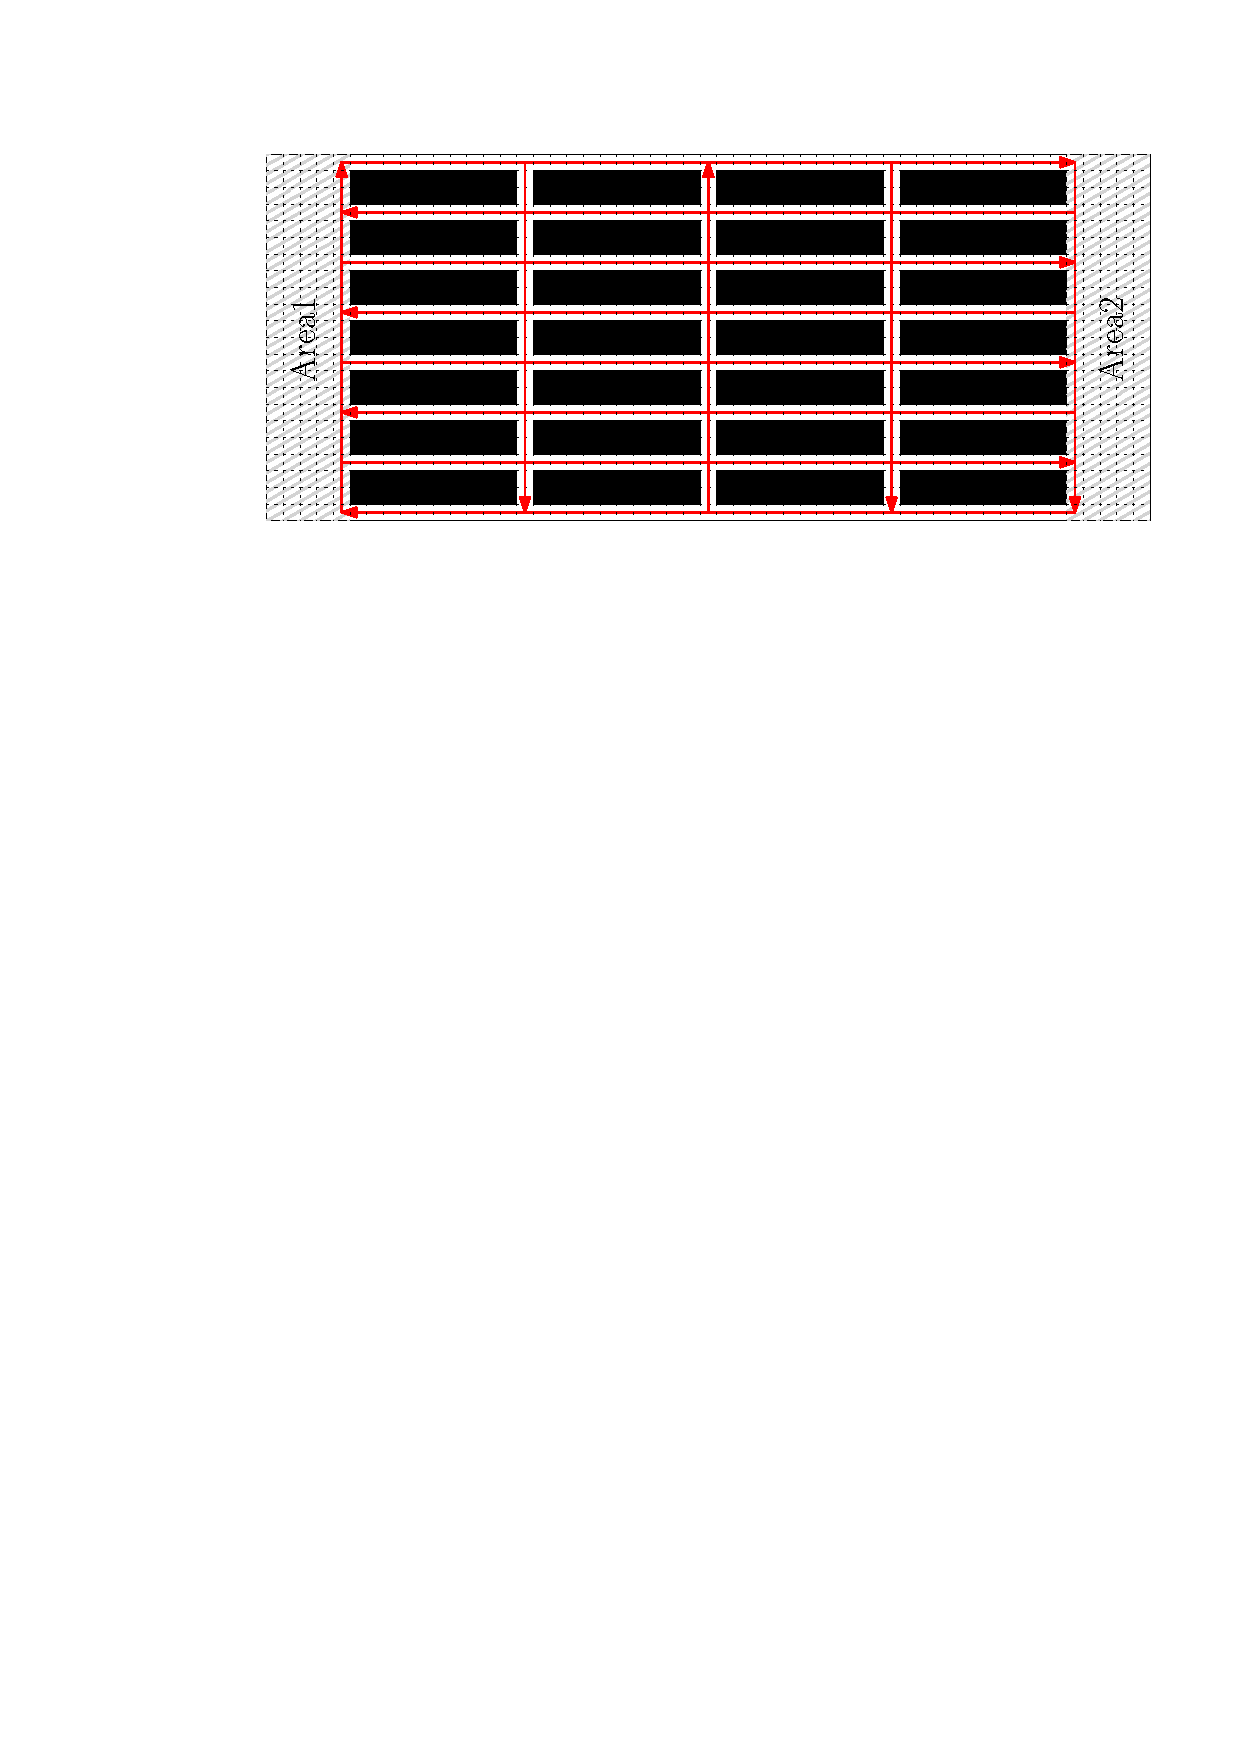
\includegraphics[width=\columnwidth]{Figs/Kiva_Domain.pdf}
  \caption{Kiva-like domain on which we compare ECBS($w$) and ECBS($w_1$)+HWY($2.0$).}
  \label{exampleKiva_fig}
\end{figure}

We presented a new bounded-suboptimal MAPF approach that takes advantage of
additional inputs that represent a highway and a parameter $w$. It uses the
highway to derive new $w$-admissible heuristic values that encourage path
finding to return paths that include the edges of the highway. The level of
encouragement increases with $w$. Our new bounded-suboptimal variants of CBS
and ECBS($w$), called CBS+HWY($w$) and ECBS($w_1$)+HWY($w_2$), encourage a
global behavior of the agents that avoids collisions. On the theoretical side,
we developed a simple approach that uses highways for MAPF and provides
suboptimality guarantees. On the experimental side, we demonstrated that
ECBS($w_1$)+HWY($w_2$) can decrease the runtimes and solution costs of
ECBS($w$) in Kiva-like domains with many agents if the highway captures the
problem structure well.

In future work, we plan to develop approaches that determine good highways
automatically, investigate whether inflating the edge costs of the given graph
(by increasing the costs of highway edges to $w$) in addition to inflating
the heuristic values provides additional benefits, figure out whether
penalizing movement costs against highway edges (similar to direction maps
\cite{JS:AIIDE:08}) helps to improve the performance of our MAPF approaches
while continuing to provide suboptimality guarantees, extend
ECBS($w_1$)+HWY($w_2$) to split the user-provided suboptimality bound $w$
dynamically between $w_1$ and $w_2$ (similar to how ECBS($w$) splits the
suboptimality bound $w$ dynamically between the high-level and low-level
searches), and explore highways in the context of other MAPF algorithms, such
as M* and inflated M*.

\section{Acknowledgments}

We thank Maxim Likhachev and Michael Phillips for helpful discussions. We also
thank Ariel Felner, Guni Sharon, and Maxim Barer for their CBS and ECBS($w$)
source code, which we used in our experiments. Our research was supported by
NSF under grant numbers 1409987 and 1319966. The views and conclusions
contained in this document are those of the authors and should not be
interpreted as representing the official policies, either expressed or
implied, of the sponsoring organizations, agencies or the U.S. government.

% References and End of Paper
\bibliography{Refs}
\bibliographystyle{aaai}
\end{document}

